\chapter{Development of Synthetic Smokers}
\label{ch:synthetic-smoker}

The iterative development of MIBot, as described in Chapter~\ref{ch:mibot})required that we extensively test it after every change in its prompt. To automate the testing of some aspects of the chatbot's behaviour, we started the development of ``synthetic smokers.''\footnote{It is worth mentioning that we also utilized human role-playing as smokers during our testing of MIBot.} A Synthetic Smoker, in the context of this research, is a prompted instance of an LLM tasked to simulate the behaviour, language, and psychological responses of a human smoker engaged in a counselling session.

This chapter details the conceptualization, iterative development, and validation of these synthetic agents.

\section{Objectives and Overview}
\label{sec:synthetic-smoker-goals}

The overarching goal of developing synthetic smokers is to create realistic and controllable stand-ins for human participants. This endeavour serves two primary objectives:

\begin{enumerate}
    \item \textbf{Testing Automated Systems:} Synthetic smokers provide a platform for the rapid iterative development and testing of automated counselling chatbots. By simulating interactions, developers may identify weaknesses, refine conversational strategies, and assess potential efficiency without the logistical overhead of recruiting human subjects for every iteration.
    \item \textbf{Training Human Clinicians:} In the role of standardized patients, synthetic smokers can be used to train novice clinicians. They offer a consistent experience and can be programmed to simulate specific challenging scenarios or diverse demographic profiles, which could help trainees receive varied practice opportunities.
\end{enumerate}

The development of a truly representative synthetic smoker poses a scientific challenge. It requires not only the generation of coherent dialogue but the accurate embodiment of specific human attributes ranging from demographics to complex psychological states like resistance to change. Crucially, the validation of these synthetic agents (i.e., proving that they behave realistically according to their installed attributes) is exceptionally difficult, as establishing the \textit{construct validity} of behavioural measurements remains a persistent challenge; that is, it is difficult to ensure that an instrument truly measures the specific psychological attribute it purports to assess \cite{Cronbach1955}.


\section{Goals for a Synthetic Smoker}
\label{sec:synthetic-smoker-ideal}

In an ideal scenario, a synthetic smoker would be indistinguishable from a human participant within the constrained context of a smoking cessation counselling session. This requires the synthetic agent to possess a defined set of attributes and for those attributes to be reliably reflected in its interactions and behaviours.

We conceptualize a synthetic smoker based on a collection of attributes that define a human smoker. These attributes can be broadly categorized as:

\begin{itemize}
    \item \textbf{Demographic:} age, sex, education level, cultural background, etc.
    \item \textbf{Behavioural:} smoking history (e.g., Heaviness of Smoking Index (HSI)), previous quit attempts, verbosit, etc.
    \item \textbf{Psychological:} resistance to change, motivation levels (e.g., operationalized by pre-conversation readiness rulers), underlying values.
\end{itemize}

A successful system (or methodology) for creating synthetic smokers must produce agents that exhibit both high \emph{fidelity} and \emph{representativeness}.

\textbf{Fidelity} refers to the requirement that any attribute installed in the synthetic smoker must be demonstrably evidenced by its language and behaviour. For example, if a synthetic smoker is installed with high resistance, its dialogue should contain more sustain talk than change talk. The core challenge of this research is to develop methods to install these attributes and subsequently validate that this installation was successful.

\textbf{Representativeness} encompasses two key requirements:

\begin{enumerate}
    \item The system must generate a diverse range of smokers whose attributes mirror the variability of the target real-world population. It must avoid the bias of over-representing a narrow or easily simulated archetype at the expense of mirroring the population's true statistical makeup. This may happen for a variety of reasons. For example, if the system is built on biased data, it may fail to generate a statistically accurate population.

    \item The smokers created by the system should exhibit uniform fidelity, i.e., it should not have performance biases where specific profiles are simulated more accurately than others. A system might, for instance, be highly effective at simulating a 55-year-old, heavily dependent smoker with low motivation to quit, while failing to simulate a 22-year-old ``social smoker'' who is ambivalent about quitting. Representativeness requires that the quality of the simulation remains high across the entire spectrum of generated profiles.
\end{enumerate}



Let the collection of all relevant attributes define an $n$-dimensional \emph{attribute space}, $\mathcal{A}$. A specific smoker's profile, whether human or synthetic, is a vector $\textbf{A}$ within this space.
$$\textbf{A} = (a_1, a_2, \ldots, a_n) \in \mathcal{A}$$

The \emph{observable output space}, $\Gamma$, contains all possible outputs from a counselling session, such as conversation transcripts and survey responses. A specific session's output is an element $\gamma \in \Gamma$.
$$\gamma = \{\text{Transcript}, \text{Survey Responses}, \ldots\}$$

Human behaviour is not deterministic; a human $H$ with a given attribute vector $\textbf{A}_H$ will not produce the exact same output in every session. Instead, their behaviour is better modelled as a sample from a conditional probability distribution, $P_H(\gamma | \textbf{A}_H)$. Consequently, a synthetic smoker system, $S$, should not be a deterministic function but a model that approximates this human distribution, $P_S(\gamma | \textbf{A}_S)$. The goal is to ensure that $P_S(\gamma | \textbf{A}) \approx P_H(\gamma | \textbf{A})$.

To assess whether the system has achieved this goal, we must formalize the process of validation. For this, we define a \emph{measurement function}, $M$, that takes an output $\gamma$ and returns an estimated attribute vector $\hat{\textbf{A}}$.

$$M: \Gamma \rightarrow \mathcal{A}, \quad \text{where} \quad \hat{\textbf{A}} = M(\gamma)$$

For example, $M$ could be a set of classifiers and analytical tools that read a transcript and analyze post-conversation changes in behaviour to estimate the speaker's resistance, motivation, smoking history, etc., and produce  $\hat{\textbf{A}}$. It is worth mentioning that the measurement function $M$ is an imperfect proxy, as inferring latent constructs from observable behaviour is a persistent challenge in psychometric theory \cite{loevinger1957objective, borsboom2004concept}.

\subsection{Defining Fidelity}

Fidelity measures how accurately the observable outputs of a synthetic smoker reflect its assigned attributes. High fidelity is achieved when the attributes measured from the output, $\hat{\textbf{A}}_S = M(\gamma_S)$, are close to the input attributes, $\textbf{A}_S$. We quantify this correspondence using a distance metric, $d(\textbf{A}_S, \hat{\textbf{A}}_S)$, in the attribute space.

Given the stochastic nature of the generative system, a single instance is insufficient for evaluation. We therefore define the fidelity for a profile $\textbf{A}_S$ as the \emph{expected distance} between the input and measured attributes over the distribution of all possible outputs.
$$\mathcal{F}(\textbf{A}_S) = \mathbb{E}_{\gamma_S \sim P_S(\gamma | \textbf{A}_S)}[d(\textbf{A}_S, M(\gamma_S))]$$
A lower value of $\mathcal{F}(\textbf{A}_S)$ indicates higher fidelity. The objective of the system, then, is to minimize this value across all possible profiles.

In practice, one may not need $M$ to calculate the fidelity, nor is it necessary to recover the full attribute vector $\textbf{A}$. Instead, a more pragmatic approach is to validate individual attributes by demonstrating a strong correlation between their installed values and corresponding, measurable features in the output $\gamma$. For example, to validate the `resistance to change' attribute, one can measure a proxy like the percentage change talk (\%CT) in the transcript. Evidence of fidelity would be a strong, negative correlation between the installed resistance level and the observed change talk across a cohort of synthetic agents. This correlation-based method is more feasible than developing a comprehensive measurement function $M$.

\subsection{Defining Representativeness}

Representativeness ($\mathcal{R}$) ensures that the synthetic population is both a statistically accurate and a consistently well-simulated reflection of the real-world population. It comprises two distinct components.

\subsubsection{Distributional Representativeness}

The first requirement, which we term \textbf{distributional representativeness} ($\mathcal{R}_{dist}$), is that the statistical makeup of the generated synthetic smokers matches that of the target human population. Let $P_H(\textbf{A})$ be the true probability distribution of attribute vectors in the target population. If we generate synthetic agents using a distribution $P_S(\textbf{A})$, this component is high when $P_S(\textbf{A})$ is close to $P_H(\textbf{A})$. We can measure this similarity using the \emph{Kullback-Leibler (KL) Divergence}:
$$\mathcal{R}_{dist} = D_{KL}(P_H(\textbf{A}) \,||\, P_S(\textbf{A})) = \sum_{\textbf{A} \in \mathcal{A}} P_H(\textbf{A}) \log\frac{P_H(\textbf{A})}{P_S(\textbf{A})}$$
A system with high distributional representativeness will minimize this divergence, ensuring that the generated population is not biased towards easily simulated archetypes. Alternatively, to assess whether the system's outputs preserve the population's statistical distribution, one can compare the original input distribution, $P_H(\textbf{A})$, to the distribution of attributes measured from the synthetic agent's final output, $P_S(M(\gamma_S))$.

The KL divergence is formulated to measure the distortion between the intended input attributes and the measured output attributes:
$$\mathcal{R}_{dist-M} = D_{KL}(P_H(\textbf{A}) \,||\, P_S(M(\gamma_S)))$$
$$= \sum_{\textbf{A} \in \mathcal{A}} P_H(\textbf{A}) \log\frac{P_H(\textbf{A})}{P_S(M(\gamma_S)=\textbf{A})}$$
Here, $P_S(M(\gamma_S)=\textbf{A})$ is the probability that the measured attributes from a synthetic agent's output $\gamma_S$ will equal the vector $\textbf{A}$, when the agent's input profile was drawn from the true human distribution $P_H(\textbf{A})$.

In practice, this is calculated by comparing the empirical distribution of a sample of human attribute vectors $\{\textbf{A}_i\}$ against the distribution of their corresponding measured outputs $\{\hat{\textbf{A}}_i = M(\gamma_i)\}$. This calculation assumes that $M$ faithfully extracts the attributes from $\gamma$, of which there is no guarantee. Therefore, a high KL divergence introduces an ambiguity: it may be due to the system's inadequacy in installing $\textbf{A}$, or it could be due to $M$ failing to recover $\textbf{A}$ from $\gamma$.


\subsubsection{Uniform Fidelity}

The second requirement, \textbf{uniform fidelity} ($\mathcal{R}_{unif}$), stipulates that the simulation quality should be consistent across all types of smoker profiles. The fidelity score, $\mathcal{F}(\textbf{A})$, should not be systematically better for some profiles than for others. We can measure this by calculating the \textit{variance of the fidelity score} across the distribution of real-world smokers, $P_H(\textbf{A})$:
$$\mathcal{R}_{unif} = \text{Var}_{\textbf{A} \sim P_H(\textbf{A})}[\mathcal{F}(\textbf{A})] = \mathbb{E}_{\textbf{A} \sim P_H(\textbf{A})} [(\mathcal{F}(\textbf{A}) - \bar{\mathcal{F}})^2]$$
where $\bar{\mathcal{F}}$ is the mean fidelity across the population. A system that achieves high uniform fidelity will have a value of $\mathcal{R}_{unif}$ close to zero, indicating that its performance is reliable and unbiased across the full spectrum of human smokers. Again, in practice, it is sufficient to calculate fidelity stratified by different relevant attributes (e.g., age groups, sex, ethnicity, etc.) and investigate if a certain group of synthetic agents has low fidelity.


\section{Development of Synthetic Smokers}
We began our development of synthetic smokers by prompting an LLM and providing instructions on how to behave like a smoker in a clinical setting. As we evaluated our synthetic smokers, both our approach of installation and validation evolved and informed each other. In the following sections, we describe our methodology for creating synthetic smokers along with their validation.


\subsection{The Baseline Synthetic Smoker}
\label{sec:synthetic-smoker-baseline}
The goal of the baseline synthetic smoker was t to create a conversational partner that could interact with MIBot prototypes, allowing the researchers to test conversational flow and MI adherence of MIBot in a controlled environment.


\subsubsection{Methodology}
We began with a minimal prompt instructing an LLM (initially GPT-4 Turbo) to adopt the persona of a smoker engaging in a counselling session. The prompt was kept minimal and did not provide a \emph{backstory} or specific behavioural constraints.

\begin{verbatim}
 You are a human smoker engaged in a private thirty-minute session
 with a counsellor. This is your first time talking to a therapist
 about your smoking habits... Respond to the counsellor's inquiries
 as accurately as possible...
\end{verbatim}

Since we did not install any attributes to this baseline, we were mainly looking for how it conversed with MIBot and whether it had some default attributes. We generated a small number (N=5) of conversations between this baseline synthetic smoker and an early version of the MIBot counsellor. The validation method at this stage was qualitative human inspection by the research team, including expert MI clinicians.

\subsubsection{Observations}
The transcript of the conversation between MIBot and the baseline synthetic smoker revealed two significant issues that made the synthetic smoker sound `unnatural' or atypical of a human smoker:

\begin{enumerate}
    \item Excessive Verbosity: The synthetic smoker tended to produce long, elaborate responses. This felt unnatural and resembled written prose more than spontaneous dialogue.
    \item High Agreeableness (Low Resistance): The baseline agent was overly agreeable and eager to change. This failed to simulate the ambivalence characteristic of many smokers seeking cessation support (as discussed in Chapter~\ref{ch:background}).
\end{enumerate}

These observations highlighted the necessity of explicitly controlling these attributes.

\subsection{Controlling Verbosity}
\label{sec:synthetic-smoker-verbosity}

To address the issue of excessive verbosity, we undertook a prompt engineering effort to constrain the synthetic smoker's utterance length and style.

\subsubsection{Methodology}
We modified the prompt to encourage a more natural, concise conversational style. Key additions to the prompt included:

\begin{itemize}
    \item Stylistic Guidance: Instructions such as ``Imagine you're texting a friend. Keep it casual...'' and encouraging the use of emojis.
    \item Instructions to be Concise: Directives like ``speak with more clarity rather than exhaustive detail.''
    \item Explicit Constraints: Hard constraints such as ``Number of sentences in your response must be between 1 and 4.''
\end{itemize}

\subsubsection{Validation}
To validate the effectiveness of these changes, we generated a new set of conversations ($n = 5$) using the modified prompt (``Fixed Verbosity'') and with GPT-4 turbo (temperature $=1.0$) and compared them against the baseline prompt (``Default Verbosity''). We also compared these results against human-human MI conversations from the High-Quality and Low-Quality Counselling (HLQC) datasets~\citep{perez-rosas-etal-2019-makes}.

\subsubsection{Results}
The prompt modifications significantly reduced the verbosity of the synthetic smoker. Figure~\ref{fig:verbosity-comparison} illustrates the distribution of volley lengths (in terms of number of words).


\begin{figure}[htpb]
    \centering
    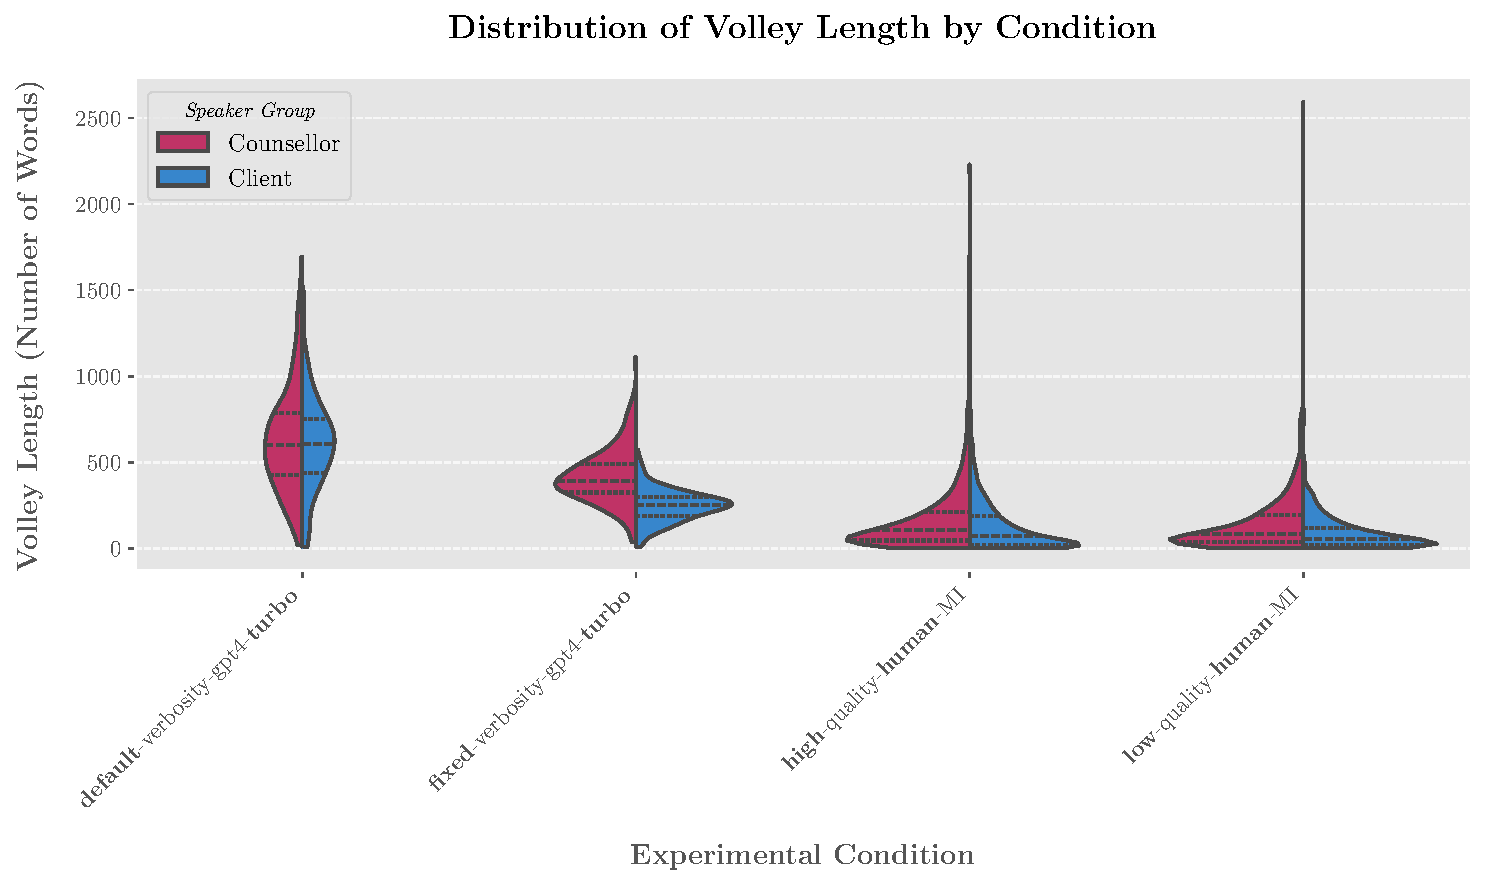
\includegraphics[width=0.9\textwidth]{fig/utterance_length_violin_plot.pdf}
    \caption[Comparison of volley length distributions for default and fixed-verbosity synthetic smokers.]{Comparison of utterance length distributions for default and fixed-verbosity synthetic smokers. The fixed-verbosity prompt successfully reduced the synthetic smoker's utterance length to better align with humans (\texttt{high-quality-human-MI}). }
    \label{fig:verbosity-comparison}
\end{figure}

\begin{table}[ht]
\centering

\label{tab:utterance_stats}
\begin{tabular}{lrr}
\toprule
{} &  \textbf{Mean} &  \textbf{Standard} \\
\textbf{Category}                   &                        &           {Deviation}          \\
\midrule
Default Verbosity (GPT-4 Turbo) &                  618.9 &               296.3 \\
Fixed Verbosity (GPT-4 Turbo)   &                  337.8 &               157.9 \\
High-Quality Human Counselling             &                  147.0 &               172.9 \\
Low-Quality Human Counselling            &                  118.2 &               158.0 \\
\bottomrule
\end{tabular}
\caption{Mean and Standard Deviation of Utterance Length by Category.}
\end{table}

The default verbosity condition showed a wide distribution with a high median utterance length. The fixed-verbosity synthetic smokers successfully matched the distribution with humans from the HQLC dataset.

Interestingly, we observed that the counsellor bot reciprocated the client's verbosity. When the synthetic smoker spoke less, the counsellor bot also reduced its utterance length. We also verified that these prompt modifications were robust and transferable across different LLMs (GPT-4 Turbo and GPT-4 Omni).

\subsection{Installing Resistance}
\label{sec:synthetic-smoker-resistance}

Addressing the baseline smoker's high agreeableness was crucial, as addressing resistance to change is a crucial MI skill.

\subsubsection{Methodology}
We hypothesized that resistance could be installed by providing the LLM with detailed backstories emphasizing different motivations and experiences. We created two distinct personas:

\begin{itemize}
    \item High Resistance Persona: The backstory emphasized severe life stressors, repeated failed quit attempts, skepticism towards therapy, and a strong belief that it was not the right time to quit.
    \item Low Resistance Persona: The backstory described recent health concerns prompting contemplation, and an open, albeit skeptical, attitude towards change.
\end{itemize}

Using modified prompts and GPT-4 Turbo (temperature=1.0), we generated conversations (N=10 per persona) between synthetic smokers and MIBot. We employed two distinct methods to validate the installation. We also prompted these synthetic smokers to fill the readiness rulers before, after, and a week after the conversation. We did so  by prompting the synthetic smoker with the exact questions from the readiness rulers survey. Before reporting the numbers, we asked them to think and provide reasons for the numerical rating they chose, before outputting the rating (a technique called chain-of-thought prompting)

\subsubsection{Validation}

\begin{enumerate}
    \item Linguistic Evidence (Change vs. Sustain Talk): We analyzed the transcripts to measure the proportion of Change Talk (CT) and Sustain Talk (ST).


    \item Behavioural 
Evidence (Self-Reported Readiness): We further validated the installation by asking the synthetic smokers to complete the Readiness Ruler survey (Importance, Confidence, and Readiness; 0-10 scale) before, immediately after, and \emph{simulated} one week after the conversation.

\end{enumerate}






\subsubsection{Results} 



\begin{table}[ht!]
\centering
\begin{tabular}{@{}llll@{}}
\toprule
\textbf{Persona} & \textbf{Change Talk (\%)} & \textbf{Sustain Talk (\%)} & \textbf{Neutral (\%)} \\ \midrule
High Resistance & 31 & 44 & 25 \\
Low Resistance & 61 & 9 & 30 \\ \bottomrule
\end{tabular}
\caption{Proportion of Change Talk, Sustain Talk, and Neutral Talk for High and Low Resistance Synthetic Smokers.}
\label{tab:resistance-ct-st}
\end{table}

\begin{table}[ht!]
  \centering
  \small
  \renewcommand{\arraystretch}{1.2} % Increased spacing slightly for readability
  \resizebox{\linewidth}{!}{\begin{tabular*}{\linewidth}{@{\extracolsep{\fill}}llcccc@{}}
    \toprule
    \textbf{} & \textbf{} & \textbf{Pre-} & \textbf{Post-} & \textbf{1-week} & \textbf{} \\
       
        \textbf{Client} & & \textbf{conversation} & \textbf{conversation} & \textbf{Follow-up} & \textbf{Change from} \\
        
    \textbf{Resistance}  &  \textbf{Variable} & \textbf{mean (SD)} & \textbf{mean (SD)} & \textbf{mean (SD)} & \textbf{Baseline} \\
    \midrule
    \multirow{3}{*}{Low} & Importance & 4.6 (0.5) & 5.4 (0.9) & 6.6 (0.5) & 2.0 (0.7) \\
    & Confidence & 2.6 (0.5) & 4.2 (1.1) & 4.8 (0.4) & 2.2 (0.4) \\
    & Readiness  & 3.2 (1.1) & 5.2 (1.1) & 5.4 (0.9) & 2.2 (1.9) \\
    \midrule
    \multirow{3}{*}{High} & Importance & 2.0 (0.0) & 4.0 (0.7) & 4.6 (1.1) & 2.6 (1.1) \\
    & Confidence & 1.0 (0.0) & 2.0 (0.0) & 2.6 (0.9) & 1.6 (0.9) \\
    & Readiness  & 0.6 (0.5) & 2.6 (0.5) & 3.4 (1.1) & 2.8 (1.1) \\
    \bottomrule
  \end{tabular*}}
  \caption{Longitudinal changes in self-reported scores (0--10 scale) for importance, confidence, and readiness, stratified by client (synthetic smoker) resistance level. Values were assessed at baseline (pre-conversation), immediately post-conversation, and at 1-week follow-up. Change scores represent the difference between baseline and 1-week follow-up. SD = standard deviation.}
  \label{tab:resistance-readiness-rulers}
\end{table}


The analysis confirmed a clear distinction between the two personas (Table~\ref{tab:resistance-ct-st}). The High Resistance smoker used significantly more Sustain Talk (44\% vs. 9\%) and less Change Talk (31\% vs. 61\%) than the Low Resistance smoker.


The readiness ruler scores demonstrated that the synthetic smokers provided responses consistent with their installed resistance levels (Table~\ref{tab:resistance-readiness-rulers}). The ``high-resistance'' synthetic smokers reported lower mean scores on all three dimensions of the readiness rulers, Interestingly, their week-later change in confidence was lower than ``low-resistance'' smokers by 0.8 points, while the change in importance and readiness was slightly higher.




This experiment also provided us with our first evidence that LLM-based synthetic smokers could self-report their smoking behaviours numerically and that the numbers were consistent with the installed attributes. We did notice, however, that the variability of scores (especially pre-conversation readiness numbers was much lower), as the only source of stochasticity among these agents was the decoding temperature of the LLM underneath.

\section{Development of Synthetic Doppelgängers}
\label{sec:synthetic-smoker-doppelgänger}

Without installing a diverse set of attributes from a target population, it became challenging to validate our development of synthetic smokers in terms of distributional representativeness and uniform fidelity. 
Therefore, we utilized the data from the feasibility study on human smoker using MIBot v6.3A (Section~\ref{sec:feasibility}) to extract installable attributes. This study provided a rich dataset of 106 MIBot-human interactions, including pre- and post-conversation readiness rulers (\emph{importance}, \emph{confidence}, \emph{readiness}), demographic data, smoking history (e.g., Heaviness of Smoking Index --- HSI), and complete conversation transcripts. Throughout the rest of the chapter, we refer to this dataset by a shorthand \textbf{MIV6.3A}.

The dataset allowed us to move away from creating synthetic smokers with an arbitrary distribution of attributes and towards a distribution drawn from MIV6.3A, where we explicitly ensured certain distributions on some attributes (e.g., we ensured the number of male and female participants to be equal before applying confidence screening). Thus, the creation of doppelgängers allowed us to validate our methodolgy more rigorously.

For the rest of our discussion, we define a doppelgänger as a synthetic smoker designed to be a ``behavioural twin'' of a specific human participant from the feasibility study, although the definition can be extended to other types of participants and studies. The goal is then to create an agent that, when exposed to MI counselling, behaves similarly to its human counterpart in terms of language use, psychological profile, and changes in readiness to quit.

Notice how the use of the doppelgänger methodolgy makes validating the fidelity of human smokers a simple approach. Rather than using a method $M$ to approximate installed attributes $\hat{\textbf{A}}_S$ from observation $\gamma_S$, we can devise a robust and clinically grounded classifier ($\textbf{C}$) that operates on $\gamma$. For example, we can calculate the fraction change talk (\%CT) from the transcripts. 

Further, we can use this classifier to find the distance $d(\textbf{C}(\gamma_H), \textbf{C}(\gamma_S))$. And since in the case of doppelgängers, $\textbf{A}_S = \textbf{A}_H$, we can approximate the fidelity as:

$$\hat{\mathcal{F}}(\textbf{A}^\textbf{C}) = \mathbb{E}_{\gamma_H \sim P_H (\gamma | \textbf{A}_H),  \:  \gamma_S \sim P_S(\gamma | \textbf{A}_H)}[d(
\textbf{C}(\gamma_H),\textbf{C}(\gamma_S)
)]$$


where $\textbf{A}^\textbf{C} = \{a \in \textbf{A} \mid a \sim \textbf{C}(\gamma)\}$. For example, if the correlation between \%CT of human and synthetic smokers is high, this can approximate the fidelity $\hat{\mathcal{F}}$. One drawback is that this kind of validation can only measure whether certain attributes are installed and evidenced in the language. It cannot give the complete picture of fidelity across all attributes. Hence, it approximates the fidelity over a small subset of attributes $\textbf{A}^\textbf{C}$, i.e., those attributes that are discernible by the classifier $\textbf{C}(\gamma)$.



\subsection{The Conversational Impact Modelling Experiment}
\label{sec:transcript-autoplay}
Before attempting to install attributes to doppelgängers and have them engage in novel conversations with MIBot, we needed to establish a baseline understanding of the LLM's ability to model the psychological impact of a conversation and contextualize the numerical readiness rulers with other installed attributes. We designed the ``Conversational Impact Modelling'' experiment for this purpose.

If an LLM-based synthetic smoker (a doppelgänger) is given the pre-conversation attributes of a human participant and the exact transcript of the MIBot-human conversation (acting as if the doppelgänger itself is speaking the human's lines), can it accurately report the same post-conversation readiness rulers as the human?

\subsubsection{Methodology}
\begin{enumerate}
\item Install the pre-conversation attributes of a specific human participant into the doppelgänger.
\item Feed the transcript of the actual conversation sequentially to the doppelgänger, framing it as a dialogue the doppelgänger is participating in.
\item After the conversation concludes, ask the doppelgänger to complete the post-conversation readiness rulers.
\end{enumerate}

In other words, the doppelgänger was provided with the participant's actual pre-conversation readiness rulers (importance, confidence, and readiness) and the full transcript of their conversation with the MIBot. After processing this information, the doppelgänger was asked to report its post-conversation readiness rulers.

The doppelgänger was given with the following system prompt:

\includesystemprompt{Conversational Impact Modelling Prompt}{
You are a participant in a study who is trying to quit smoking.\\
Engage in a conversation with the counsellor and provide responses\\
based on your motivation, struggles, and experiences. Your assistant\\
role is the client, and the user's role is the counsellor or\\
the researcher.\\\\
Before you talk to the counsellor, please answer the following
questions. \\\\
\quad On a scale from 0 to 10, how important is it to you right\\
now to stop smoking? Respond with a single integer between 0 (very\\
low importance) and 10 (very high importance).\\\\
...
}

To investigate the doppelgänger's reasoning process and potentially improve its accuracy, we utilized several prompting techniques:

\begin{enumerate}
\item Baseline: A standard prompt asking the doppelgänger for the post-conversation score.

\item Chain-of-Thought (CoT): An enhanced prompt that required the doppelgänger to articulate its reasoning by reflecting on the conversation's key insights, its own motivations, and any expressed shifts in perspective—before providing the final numerical score.
\end{enumerate}

We tested this methodology with multiple underlying models, including GPT-4o and Claude 3.7 Sonnet. For the Claude model, we also leveraged its native ``thinking'' feature, which allows the doppelgänger to perform internal monologue and reflection before generating a final answer, serving as a functional alternative to an explicit CoT prompt.

\subsubsection{Evaluation}
The primary evaluation metrics were the Mean Absolute Error (MAE), Mean Squared Error (MSE), and Spearman's Correlation (r) between the human-reported and doppelgänger-reported outcomes.

\subsubsection{Results}
First, to establish a performance benchmark, a simple linear regression model was created to predict post-conversation confidence using only pre-conversation confidence from the human data. This yielded an \textbf{MSE of 3.2}, representing the baseline accuracy achievable without considering the conversational content.

The Conversational Impact Modelling experiments consistently outperformed this simple baseline, demonstrating the doppelgänger's ability to extract meaningful signals from the conversation transcripts. An initial ablation study, summarized in \cref{tab:ablation_results}, reveals the importance of providing the doppelgänger with both the pre-conversation context and the transcript.



\begin{table}[ht!]
\centering

\begin{tabular}{@{}lrr@{}}
\cmidrule(r){1-2}
\textbf{Input Provided to GPT-4o} & \textbf{Mean Squared Error (MSE)} & \\
\cmidrule(r){1-2}
Transcript ONLY & 5.5 & \\
Pre-Conversation Confidence ONLY & 3.7 & \\
\textcolor{gray}{Linear Regression (Pre-Conf. $\rightarrow$ Post-Conf.)} & \textcolor{gray}{ 3.2} & \textcolor{red}{\small $\leftarrow$ Baseline} \\
Pre-Conversation Confidence + Transcript & 3.1 & \\
\textbf{Full Pre-Conversation Rulers + Transcript} & \textbf{2.9} & \\
\cmidrule(r){1-2}
\end{tabular}
\caption[Ablation Study on doppelgängers' self-reported post-conversation confidence]{Impact of Different attributes on GPT-4o-based doppelgängers' self-reported Post-Conversation Confidence. Both the pre-conversation readiness rulers and the conversation transcript are necessary for the doppelgängers to accurately report post-conversation confidence.}
\label{tab:ablation_results}
\end{table}



While metrics like MAE provide a quantitative summary, a visual comparison of the distributions reveals some discrepancies. \cref{fig:post_conf_distributions} plots the distribution of human-reported confidence scores alongside the distribution of GPT-4o-based doppleganger. Both distributions are similarly left-skewed, indicating that the model correctly identifies that most participants land in the higher-confidence range (6-10). However, the doppelgänger predictions were less varied than the human responses. The human data shows a broader plateau of high confidence across scores 6, 7, and 8, whereas the doppelgängers' exhibit a pronounced peak at a score of 7. This suggests that while the model is effective at capturing the overall positive trend, it may be less sensitive to the subtle individual differences in participants' final confidence levels, tending to revert to a more common or 'average' high-confidence outcome.



\begin{figure}[ht!]
    \centering
    \begin{minipage}{0.48\textwidth}
        \centering
        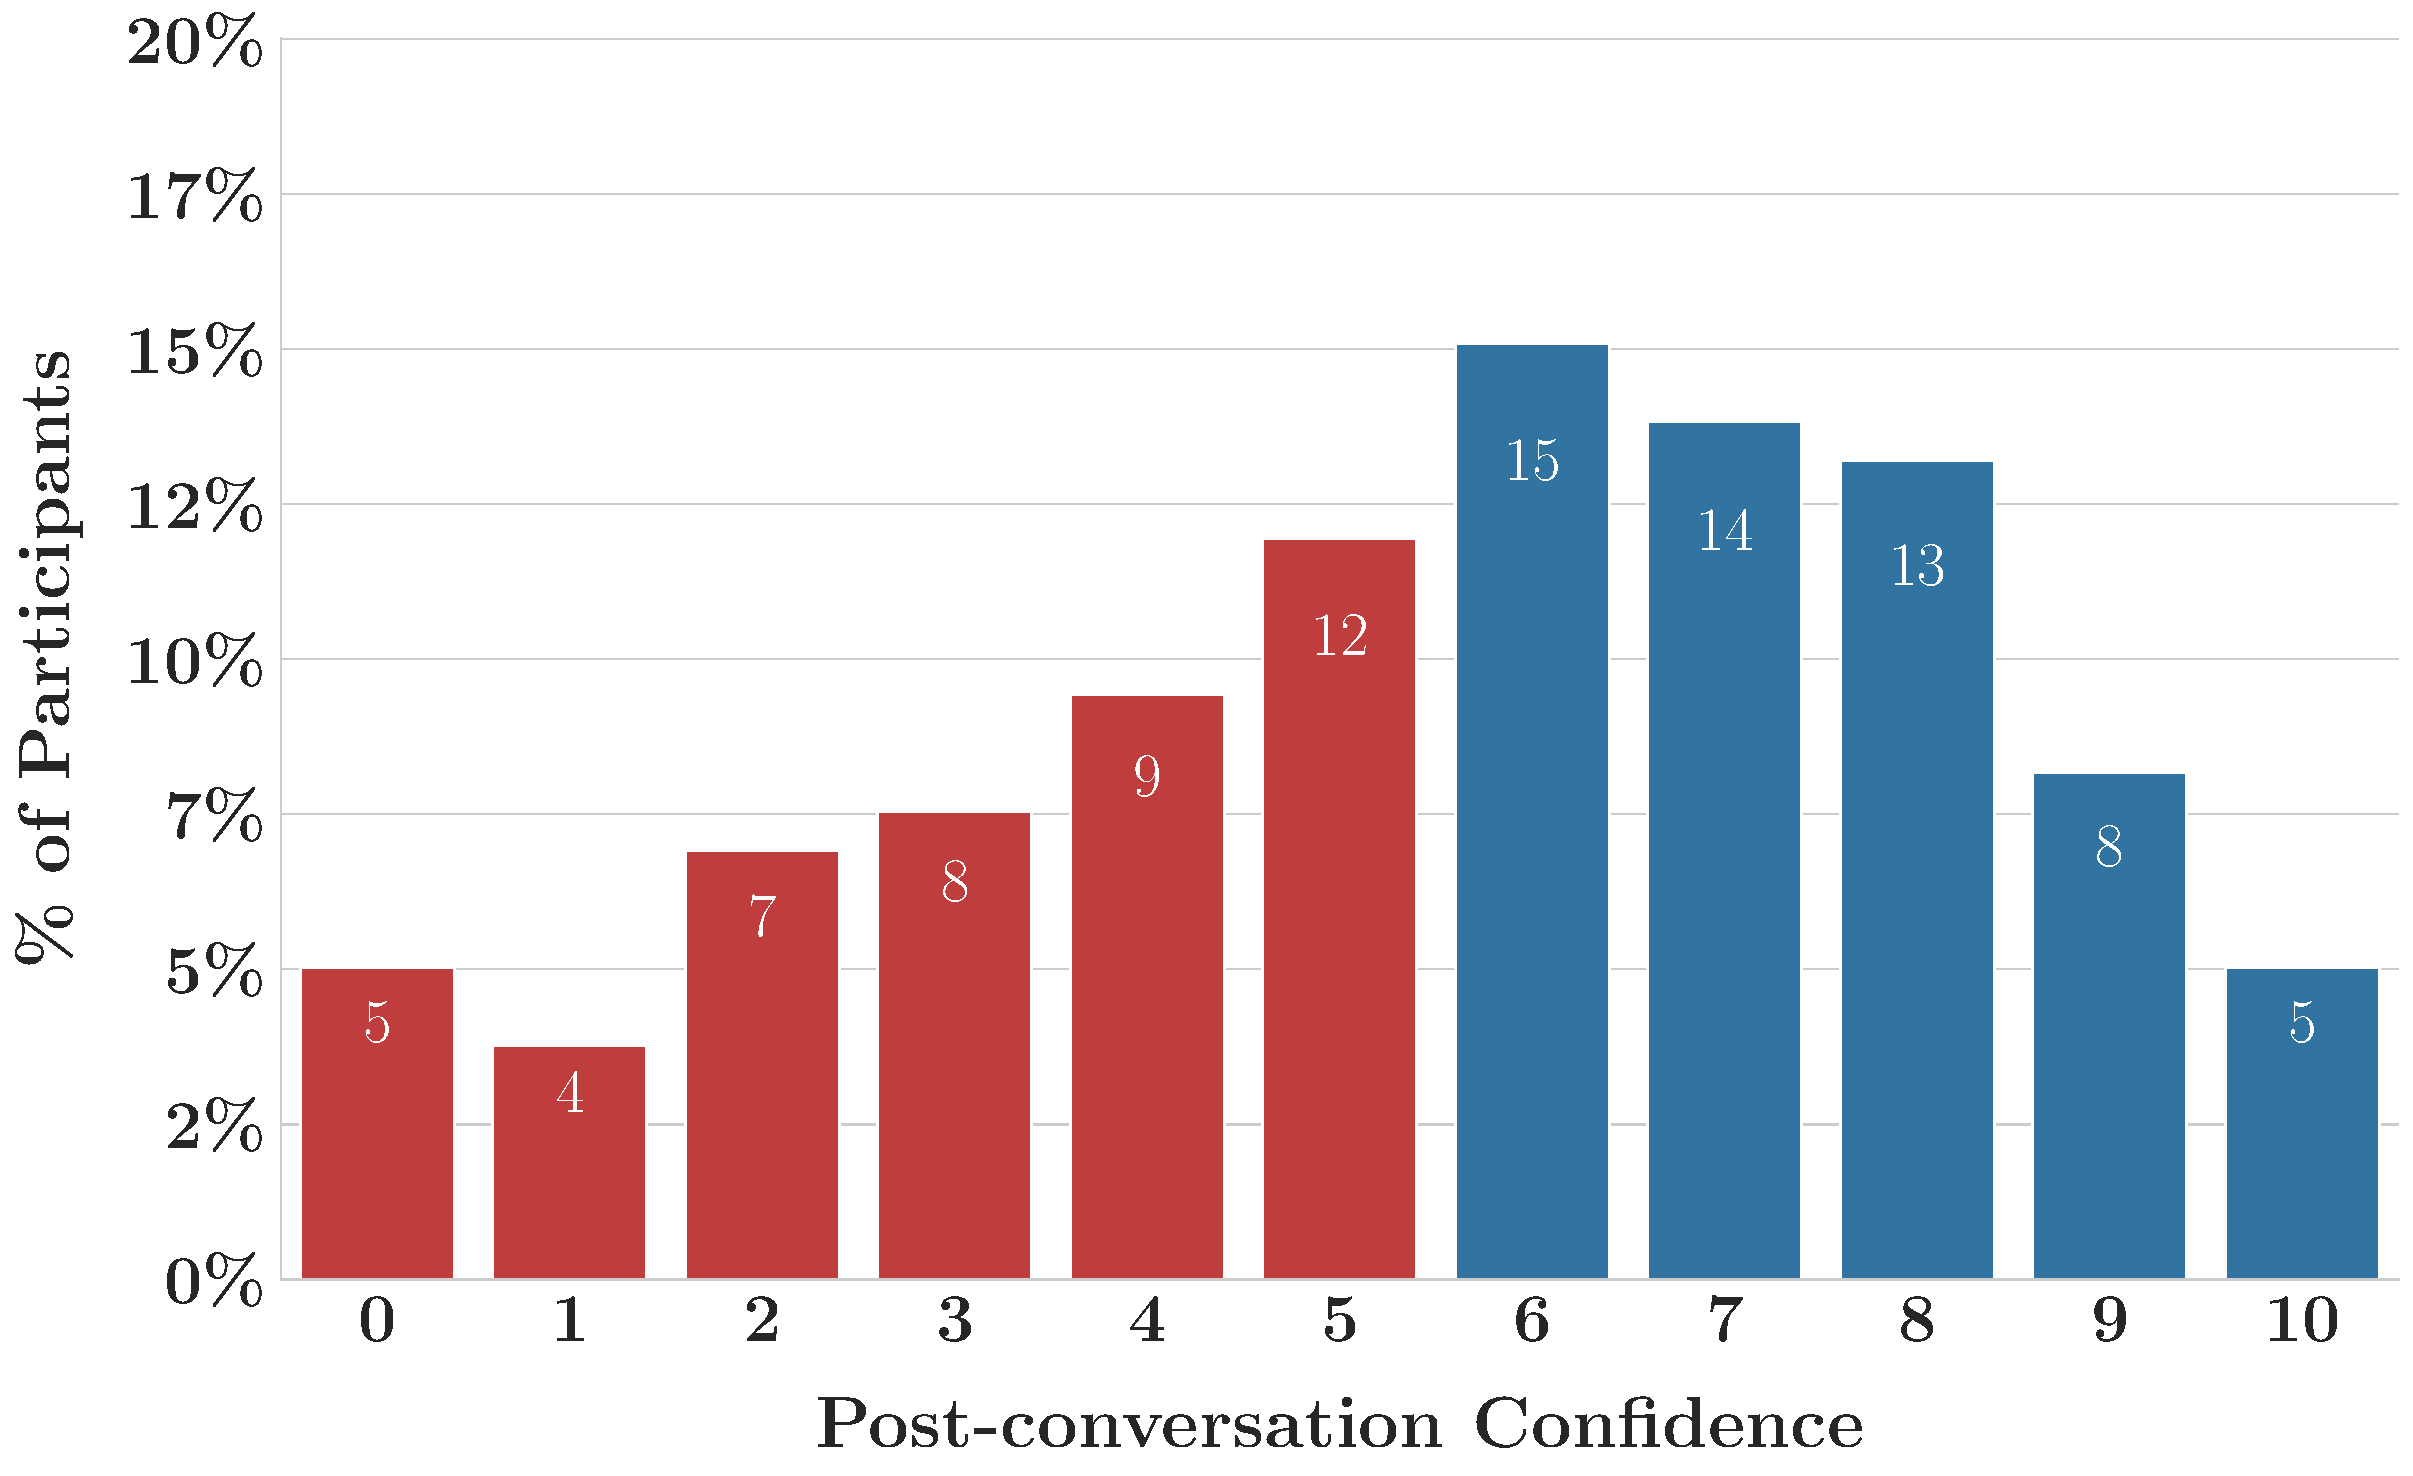
\includegraphics[width=\linewidth]{fig/post-conf-human.pdf}
        \subcaption{Human-reported post-conv. confidence scores}
        % No sub-caption needed as the main caption explains it
    \end{minipage}\hfill
    \begin{minipage}{0.49\textwidth}
        \centering
        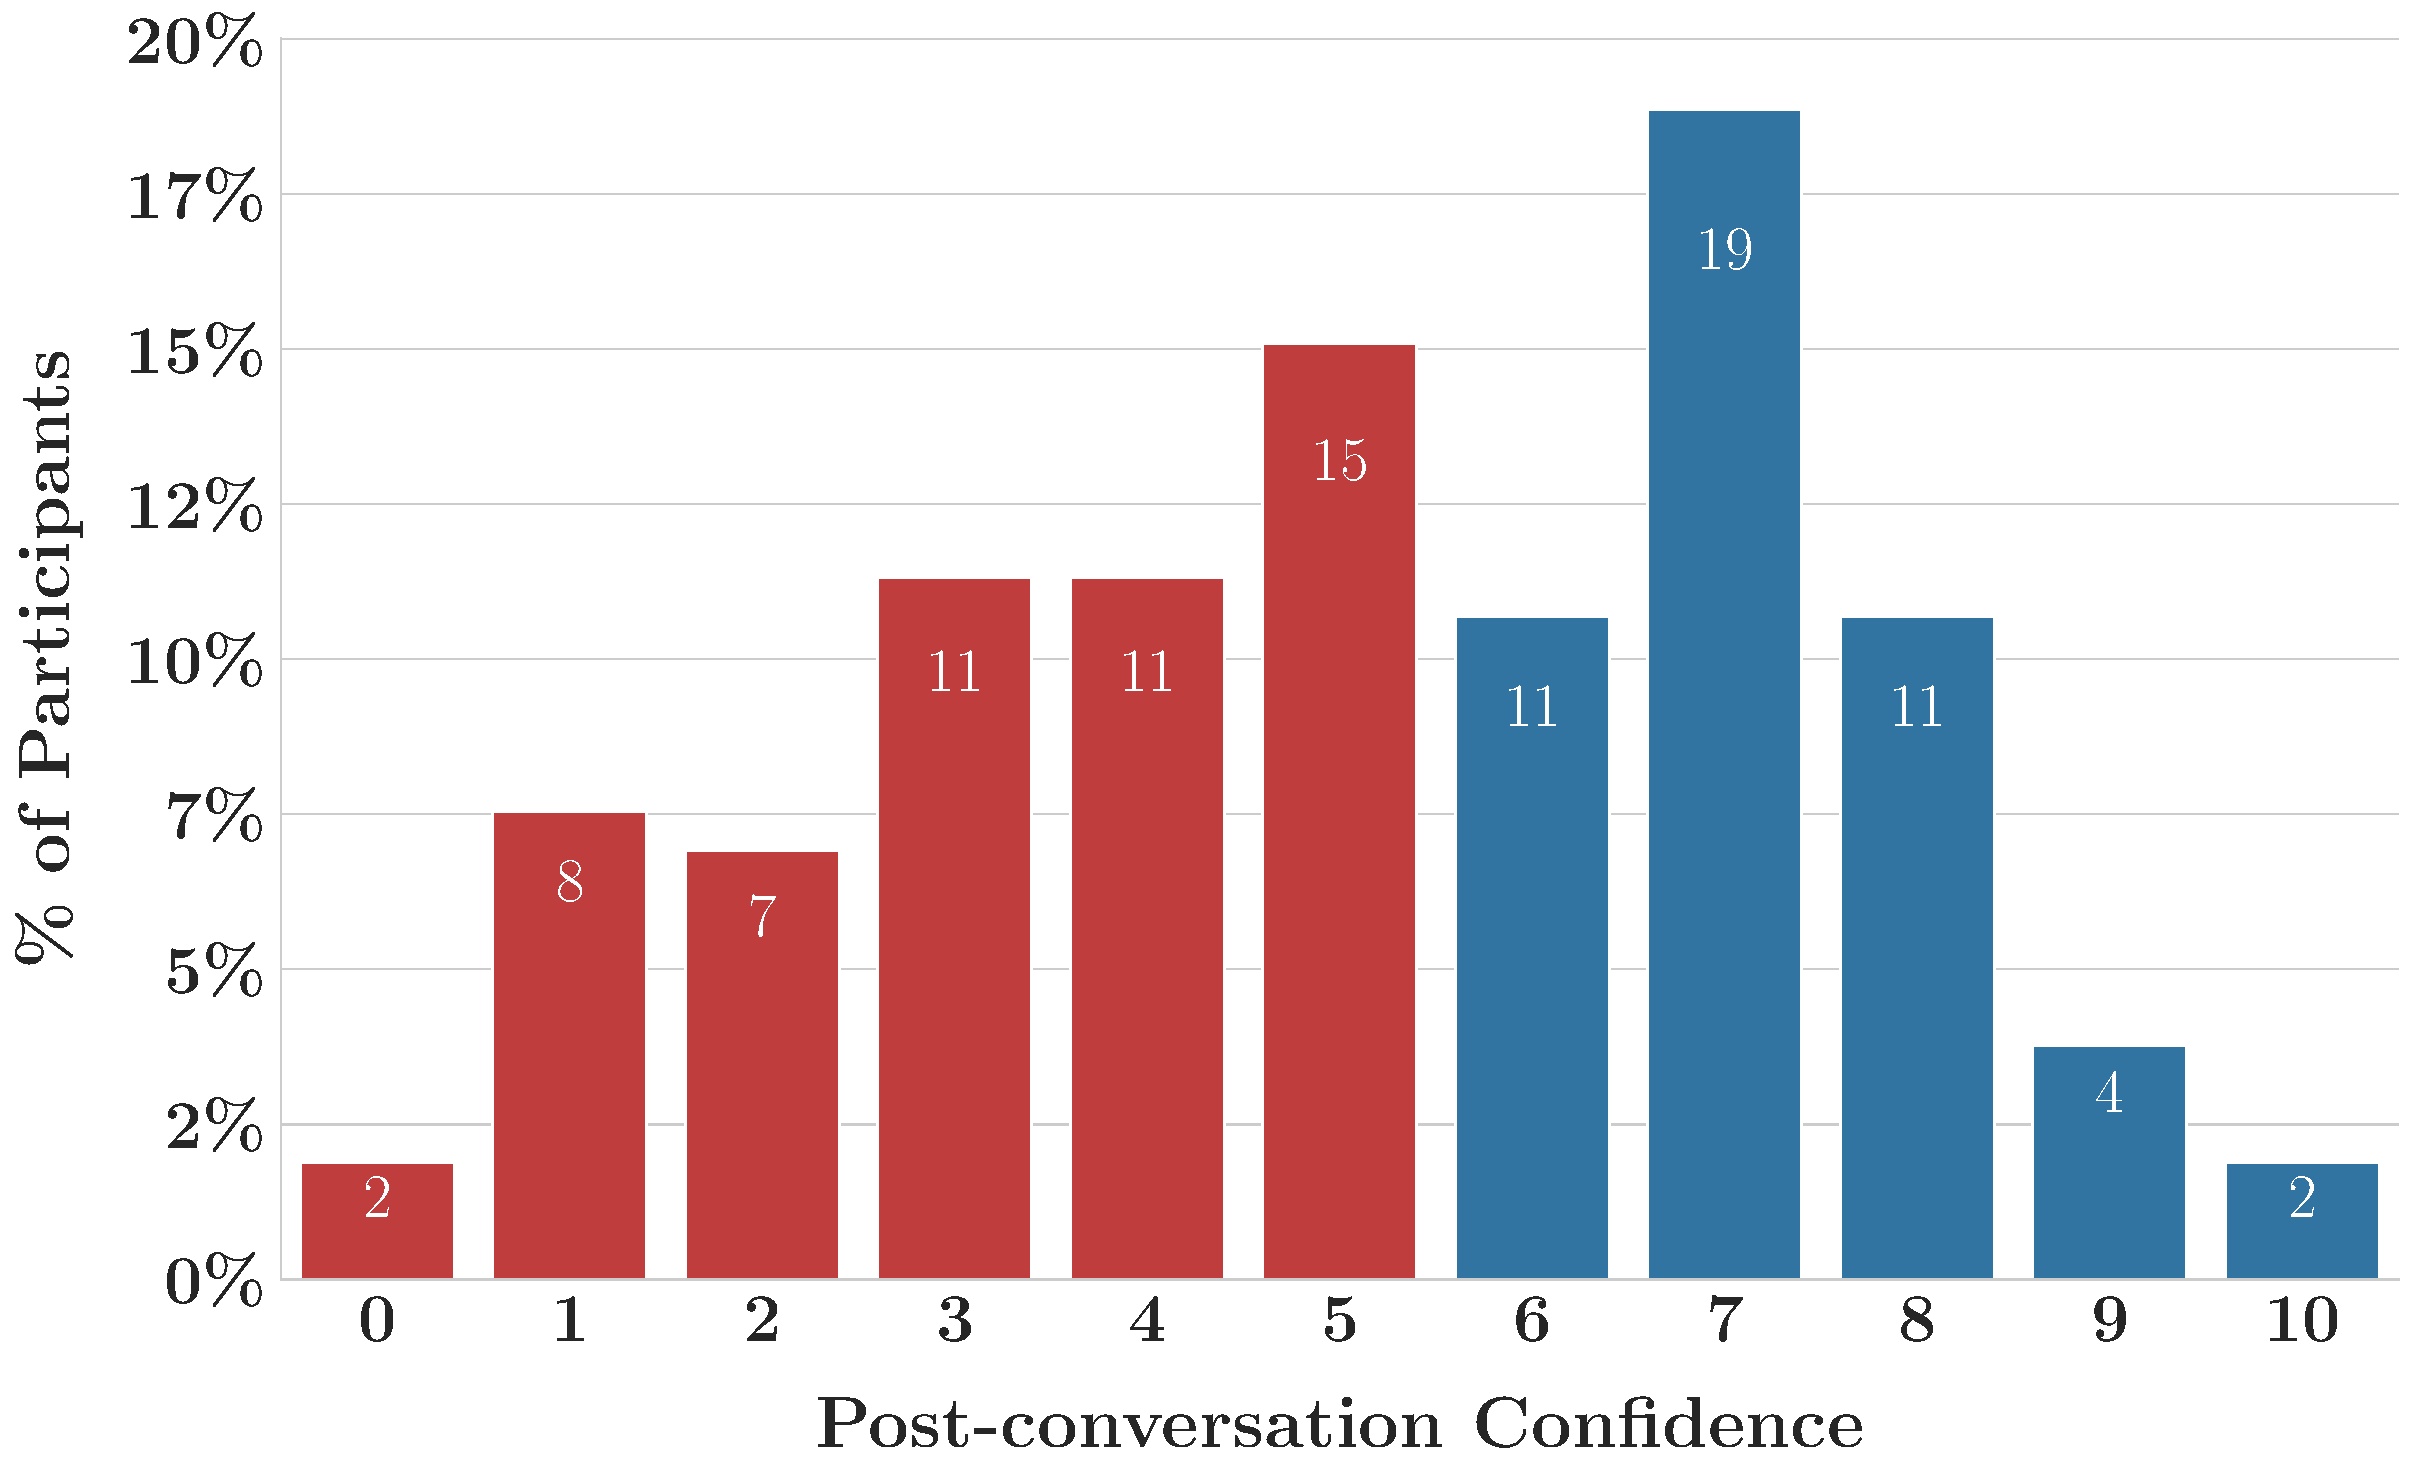
\includegraphics[width=\linewidth]{fig/post-conf-gpt4-o.pdf}
        \subcaption{doppelgänger-reported post-conv. confidence scores}
    \end{minipage}
    \caption{Distribution of post-conversation confidence scores. \textbf{Left:} Human-reported post-conversation confidence scores. \textbf{Right:} GPT-4o-based doppelgänger-reported  post-conversation confidence scores. While the overall shapes are similar, the doppelgänger's scores are more concentrated around a single peak (score of 7), whereas human responses are more distributed across several high-confidence values.}
    \label{fig:post_conf_distributions}
\end{figure}


Next, we compared the performance of different underlying models and prompting techniques used by the doppelgängers to report post-conversation confidence. The results, detailed in Table \ref{tab:model_comparison}, show that reflective prompting methods consistently improved accuracy.


\begin{table}[!ht]
\centering
\begin{tabular}{l|cccc}
\toprule
\textbf{Model} & \textbf{MAE} & \textbf{MSE} & \textbf{Correlation (r)} & \textbf{Exact Matches (\%)} \\
\midrule
GPT-4o (Baseline) & 1.2 & 3.0 & 0.7 & 31
\\
GPT-4o (CoT) & 1.2 & 2.9 & 0.7 & 30 \\
Claude 3.7 Sonnet (CoT) & 1.2 & 2.7 & 0.7 & 31 \\
\textbf{Claude 3.7 Sonnet (Thinking)} & \textbf{1.1} & \textbf{2.6} & \textbf{0.8} & \textbf{32} \\ 
\bottomrule
\end{tabular}
\caption[Model and Prompting Technique Comparison]{Comparison of different models and prompting techniques and their impact on the self-reporting of post-conversation confidence (N=159). Reflective techniques, especially Claude 3.7 Sonnet's ``thinking'' feature, yielded the best results across all metrics.}
\end{table}

The baseline GPT-4o doppelgänger achieved a strong correlation of \textbf{r=0.7} with the human-reported scores. However, the \textbf{Claude 3.7 Sonnet doppelgänger using its ``thinking'' feature achieved the lowest error (MAE=1.1, MSE=2.6) and the highest correlation (r=0.8)}.


\begin{figure}[htpb]
    \centering
    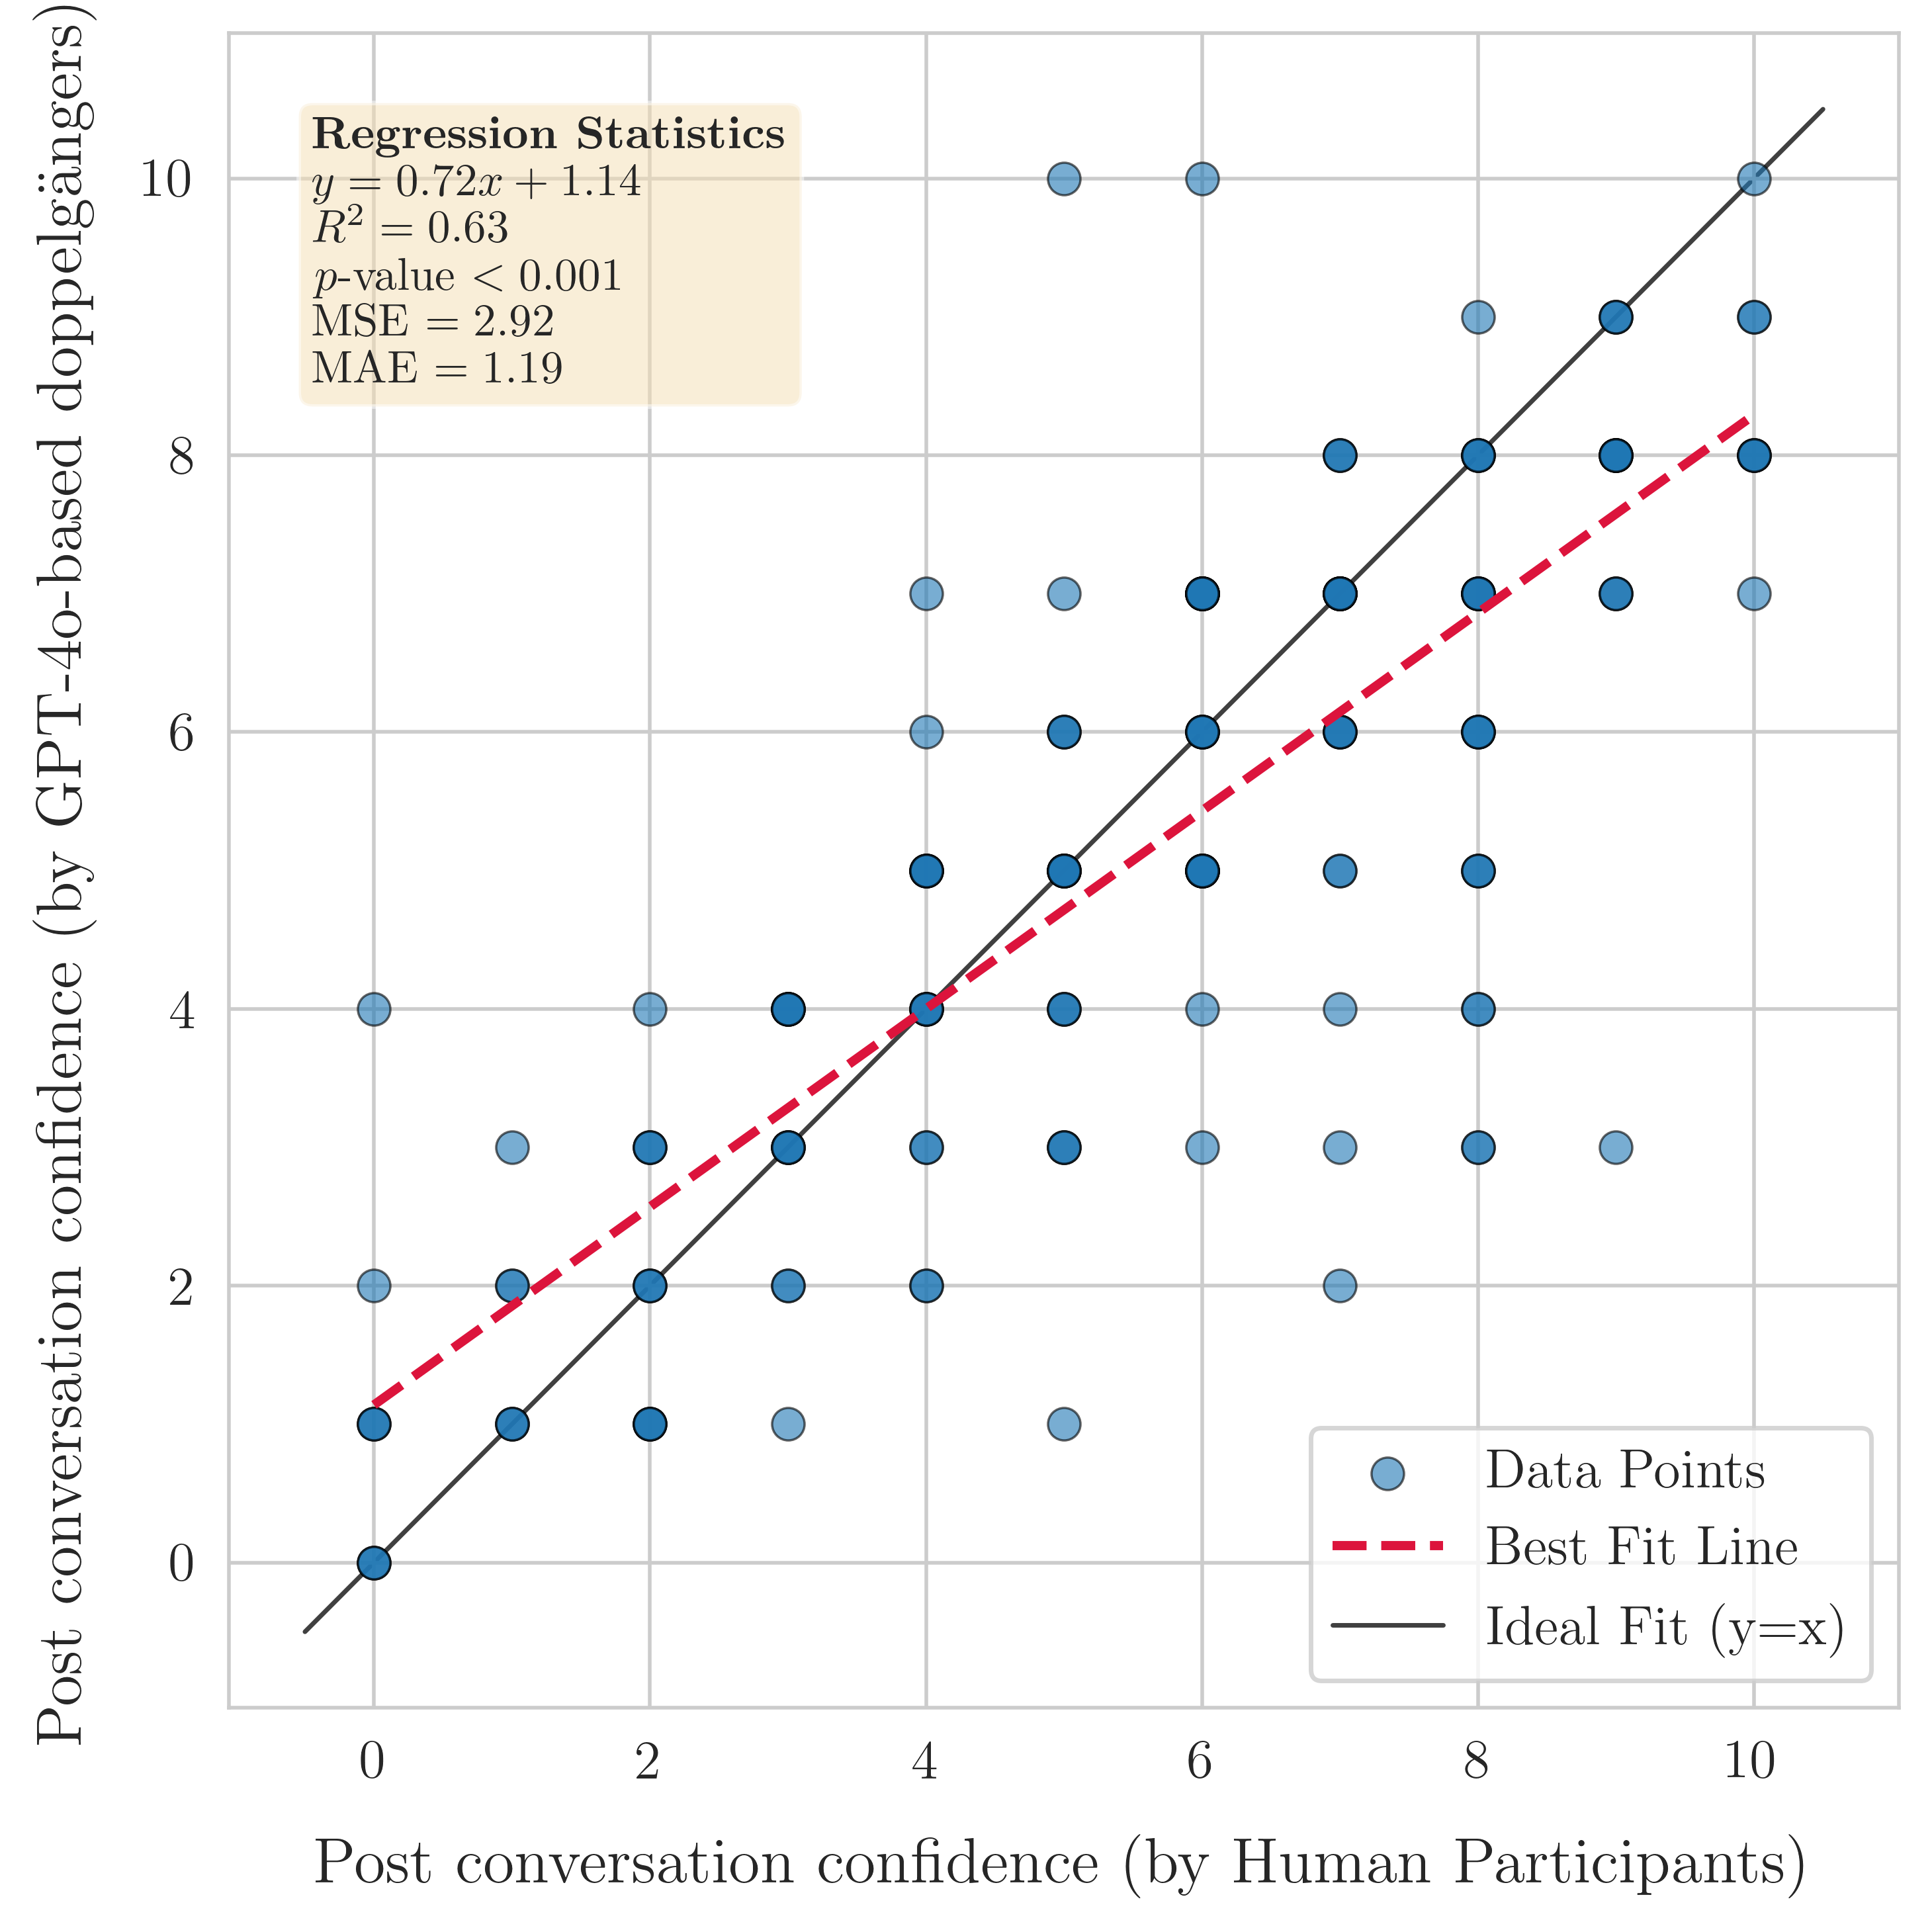
\includegraphics[width=0.5\textwidth]{fig/post_conf_gpt4o_vs_human.png}
    \caption{Scatter plot of human-reported vs. doppelgänger-reported post-conversation confidence for the baseline GPT-4o model, showing a Spearman's correlation of r=0.70. The diagonal line represents perfect agreement.}
    \label{fig:post-conf-gpt4o-vs-human}
\end{figure}


Figure~\ref{fig:post-conf-gpt4o-vs-human} visualizes the relationship between the post-conversation confidence reported by human participants and that reported by their corresponding GPT-4o-based doppelgängers. The analysis reveals a strong, statistically significant positive correlation (R 
2
 =0.63,p<0.001), indicating that the doppelgängers are generally successful in mirroring the human outcomes after processing the conversation transcript. The Mean Absolute Error (MAE) was 1.19, suggesting the doppelgänger's reported score was typically within about 1.2 points of the human's score on the 0-10 scale.

However, the plot also reveals a notable trend when comparing the best-fit line (dashed red) with the ideal fit (solid black). The regression equation (y=0.72x+1.14) shows a slope less than 1.0 and a positive intercept. This indicates a tendency towards "regression to the mean" in the doppelgänger reports. Specifically, when human participants reported very low confidence (e.g., 0-3), the doppelgängers tended to report slightly higher confidence (closer to the intercept of 1.14). Conversely, when humans reported very high confidence (e.g., 8-10), the doppelgängers tended to report slightly lower confidence. This suggests that while the directional impact of the conversation is captured well, the magnitude of the impact at the extremes might be slightly attenuated in the synthetic agents.

We further extended this analysis to include the other two readiness rulers: Importance and Readiness. The results are summarized in Table~\ref{tab:model_comparison}.




\begin{table}[!ht]
\centering
\label{tab:autoplay_results_full}
\begin{tabular}{l|cc|cc|cc}
\toprule
& \multicolumn{2}{c|}{\textbf{Post-Confidence}} & \multicolumn{2}{c|}{\textbf{Post-Importance}} & \multicolumn{2}{c}{\textbf{Post-Readiness}} \\
\textbf{Model} & \textbf{MAE} & \textbf{Corr.} & \textbf{MAE} & \textbf{Corr.} & \textbf{MAE} & \textbf{Corr.} \\ 
\midrule
GPT-4o (CoT) & 1.2 & 0.7 & 0.8 & 0.9 & 0.7 & 0.9 \\
Claude 3.7 (Thinking) & 1.1 & 0.8 & 0.7 & 0.9 & 0.9 & 0.8 \\ \hline
\end{tabular}
\caption[Multi-Ruler Conversational Impact Modelling Results]{Results of the Conversational Impact Modelling experiment across all three readiness rulers, showing MAE and Pearson Correlation. Performance was consistently strong, especially for Importance and Readiness.}
\label{tab:model_comparison}
\end{table}

Table~\ref{tab:model_comparison} summarizes the performance of the Conversational Impact Modelling experiment across all three readiness rulers. The results demonstrate high correlations (ranging from 0.7 to 0.9) across all rulers for both GPT-4o and Claude 3.7 models, affirming the robustness of the methodology.

It is interesting to note that the performance metrics for post-importance and post-readiness are generally stronger than those for Post-Confidence. For example, the correlations for Importance (0.9 for both models) are notably higher, and the MAEs lower, than for confidence. This suggests that the doppelgängers found it easier to accurately model the conversational impact on a participant's sense of importance and readiness to quit than on their self-efficacy (confidence) in their ability to do so. Overall, the Claude 3.7 model utilizing its ``thinking'' feature demonstrated slightly better performance in modelling confidence (Corr. 0.8, MAE 1.1) compared to GPT-4o (Corr. 0.7, MAE 1.2).



This experiment served as a confidence check on the doppelgänger's ability to infer the psychological state resulting from the conversation. The underlying model possesses the necessary reasoning capabilities to allow the doppelgänger to understand how the conversational dynamics influenced the participant's motivation and confidence. This serves as a baseline to confirm the doppelgänger's internal consistency before attempting to generate the conversation itself.



\section{Experiments with Incremental Installation of Attributes}
Having gained insights into LLMs' ability to model conversations and their intuitive understanding of numerical attributes such as readiness rulers, we set out to systematically install attributes to LLM-based synthetic smokers and validate their installation. Recall from our discussion on the benefits of creating doppelgängers (\cref{sec:synthetic-smoker-doppelgänger}). They provide a way to approximate the fidelity of installation and make the validation of synthetic agents easier. We can approximate the fidelity of synthetic smokers with the correlation between some metric on the observable outer space (e.g., transcripts) of doppelgängers and their human twins. As an example, to validate whether the behavioural attribute of resistance to change has been successfully installed, we can analyze the transcripts from both humans and their doppelgängers, and calculate the correlation between \% Change Talk (\%CT) exhibited by both groups. A high correlation would then suggest a successful installation of this attribute.


\subsection{Percentage Change Talk: The Key Metric for Validating Behavioural Fidelity}

To validate the synthetic smokers developed using the doppelgänger method, we needed an objective metric that could measure the smokers' level of motivation from their language.
We identified the Percentage Change Talk metric (also referred to as Change Fraction or CF, calculated as CT / (CT + ST)) to fit our requirements as it is grounded in the client's language and is strongly associated with behavioural change outcomes in MI \cite{Barnett2014,Houck2018,Moyers2009,Baer2008}.
Furthermore, we tested if \%CT is a valid proxy for a client's internal state, i.e., if it correlates with established metrics of readiness in human participants.

We analyzed the data from MIV6.3A ($N=106$ participants). The analysis confirmed strong, statistically significant correlations between \%CT and all readiness rulers (Table~\ref{tab:ct-correlation}). For example, the correlation with post-conversation confidence was 0.41 ($p < 0.0001$). These results motivated us to use \%CT as a primary metric for validating the installation of behavioural attributes in the synthetic smoker.


\begin{table}[!ht]
\centering
\begin{tabular}{@{}lr@{}}
\toprule
\textbf{Attribute} & \textbf{Correlation with \%CT} \\
\midrule
Pre-conversation Importance & 0.47$^{****}$ \\
Pre-conversation Confidence & 0.29$^{**}$ \\
Pre-conversation Readiness & 0.46$^{****}$ \\
\midrule
Post-conversation Importance & 0.49$^{****}$ \\
Post-conversation Confidence & 0.41$^{****}$ \\
Post-conversation Readiness & 0.48$^{****}$ \\
\midrule
Change in Importance (Post - Pre) & 0.12 \\
Change in Confidence (Post - Pre) & 0.24$^{**}$ \\
Change in Readiness (Post - Pre) & 0.06 \\
\midrule
CARE (Perceived Empathy) & 0.15 \\
Previous number of quit attempts & 0.09 \\
Age & -0.11 \\
Number of cigarettes per day & -0.04 \\
HSI (Heaviness of Smoking Index) & -0.15 \\
\bottomrule
\multicolumn{2}{l}{\footnotesize{**** $p < 0.0001$, *** $p < 0.001$, ** $p < 0.01$, * $p < 0.05$}.}
\end{tabular}
\caption{Correlation between Percentage Change Talk (\%CT) and Human Smoker Attributes in the MIBot Dataset (N=115).}
\label{tab:ct-correlation}
\end{table}



\subsection{Process of Creating doppelgängers}
The doppelgänger methodology uses a dataset of installable human attributes (e.g., MIV6.3A containing attributes of human smokers) to build and validate synthetic smokers. The process involves:

\begin{enumerate}
    \item Attribute Installation: Instantiating a synthetic smoker, $S_i$, by installing the known attributes of a specific human participant, $H_i$, from the dataset. $A_S = A_H$. These attributes may include demographics, HSI, self-reported survey responses, etc.
    \item Simulation: The synthetic smoker $S(A_H)$ interacts with the same counsellor (MIBot in our case) that the original human interacted with.
    \item Comparison: The output of the synthetic smoker, $\gamma_S$, is compared with the actual output of the human, $\gamma_H$ (See \cref{sec:synthetic-smoker-doppelgänger})
\end{enumerate}



The overall workflow for creating and validating doppelgängers using this comparative method is illustrated in Figure~\ref{fig:doppelgänger-creation-process}.



We created a set of doppelgängers (N=20) by sampling 20 human participants from MIV6.3A. Then we conducted a series of experiments on these doppelgängers. In each experiment, we installed a subset of attributes to the doppelgängers via \emph{prompting} and did not add any backstories to their prompt.

\includesystemprompt{Example of Attribute Installation in doppelgänger Prompts}{
You are a participant in a study who is trying to quit smoking. Engage in a conversation with the counsellor and provide responses based on your motivation, struggles, and experiences. Your assistant role is the client, and the user's role is the counsellor or the \\ researcher. Always try to respond in fewer than 200 characters. \\\\
About you: You are a 30-year-old female. You typically smoke 25 cigarettes per day. After you wake up, you smoke your first cigarette within 5 minutes. In the past week, you have not made any quit attempts.\\\\
Before speaking to the counsellor, you have rated your motivation to quit as follows (on a scale from 0 to 10): Importance: 2, Confidence: 0, Readiness: 4. \\\\
You talk about changing your smoking behaviour 46\% of the time.
...
}

\subsubsection{Methodology}
Before starting our series of experiments, we sorted the set of all installable attributes based on their correlation with \%CT. We hypothesized that a high correlation between an attribute and \%CT would mean that the attribute has a bigger impact on the client's behavioural language. Let us call this sorted list of attributes $\mathbf{A'}$. 

$$
\begin{aligned}
{\textbf{A}}^{'} = \{ & \text{pre-conversation importance,} \\
                     & \text{pre-conversation readiness,} \\
                     & \text{age,} \\
                     & \text{sex,} \\
                      & \text{pre-conversation confidence,} \\
                     \cdots \}
\end{aligned}
$$

The experiment then proceeds by incrementally adding attributes from this sorted list, and at each step, measuring the fidelity of the resulting doppelgängers. Fidelity is operationalized as the correlation between the Percentage Change Talk (\%CT) of the human participants and their corresponding doppelgängers. The process is detailed in Algorithm~\ref{alg:incremental_installation}.

{ 
\setstretch{1.25}
\begin{algorithm}[H]
    \caption{Incremental Attribute Installation and Fidelity Validation}
    \label{alg:incremental_installation}
    \begin{algorithmic}[1]
        \Require Human dataset $\mathcal{D} = \{ (H_i, \mathbf{A}_{H_i}, \gamma_{H_i}) \}_{i=1}^N$ containing human participants, their full attribute vectors, and conversation transcripts.
        \Require Sorted list of attributes $\mathbf{A'} = (a'_1, a'_2, \dots, a'_m)$ ordered by hypothesized relevance.\vspace{5pt}
        \State Initialize $\mathbf{A}_{\text{installed}} \leftarrow \emptyset$ \Comment{The set of attributes to install}
        \State Initialize $C \leftarrow ()$ \Comment{An empty list to store correlation results}

        \For{$k \leftarrow 1 \text{ to } m$} \Comment{Iterate through the sorted list of attributes}
            \State $\mathbf{A}_{\text{installed}} \leftarrow \mathbf{A}_{\text{installed}} \cup \{a'_k\}$ \Comment{Add the next attribute}
            
            \State Initialize $\mathbf{V}_{\text{human\_CT}} \leftarrow ()$ and $\mathbf{V}_{\text{synth\_CT}} \leftarrow ()$ \Comment{Vectors for \%CT scores}
            
            \For{$i \leftarrow 1 \text{ to } N$} \Comment{For each human participant in the dataset}
                \State $\mathbf{A}_{\text{subset}} \leftarrow \mathbf{A}_{H_i} |_{\mathbf{A}_{\text{installed}}}$ \Comment{Filter attributes for the current iteration}
                \State $S_i \leftarrow \mathcal{S}(\mathbf{A}_{\text{subset}})$ \Comment{Instantiate the synthtic smoker $S_i$ with the given parameters}
                \State Simulate a conversation between $S_i$ and MIBot to generate transcript $\gamma_{S_i}$.
                
                \State Calculate human \%CT: $c_{H_i} \leftarrow \text{\%CT}(\gamma_{H_i})$
                \State Calculate synthetic \%CT: $c_{S_i} \leftarrow \text{\%CT}(\gamma_{S_i})$
                
                \State Append $c_{H_i}$ to $\mathbf{V}_{\text{human\_CT}}$
                \State Append $c_{S_i}$ to $\mathbf{V}_{\text{synth\_CT}}$
            \EndFor
            
            \State Calculate the correlation for the current attribute set: $\rho_k \leftarrow \text{Correlation}(\mathbf{V}_{\text{human\_CT}}, \mathbf{V}_{\text{synth\_CT}})$
            \State Append $\rho_k$ to the results list $C$.
        \EndFor
        \vspace{5pt}
        \State \Return $C$ \Comment{A list of correlations, one for each incremental step of attribute installation}
    \end{algorithmic}
\end{algorithm}
}



\begin{figure}[htpb]
    \centering
    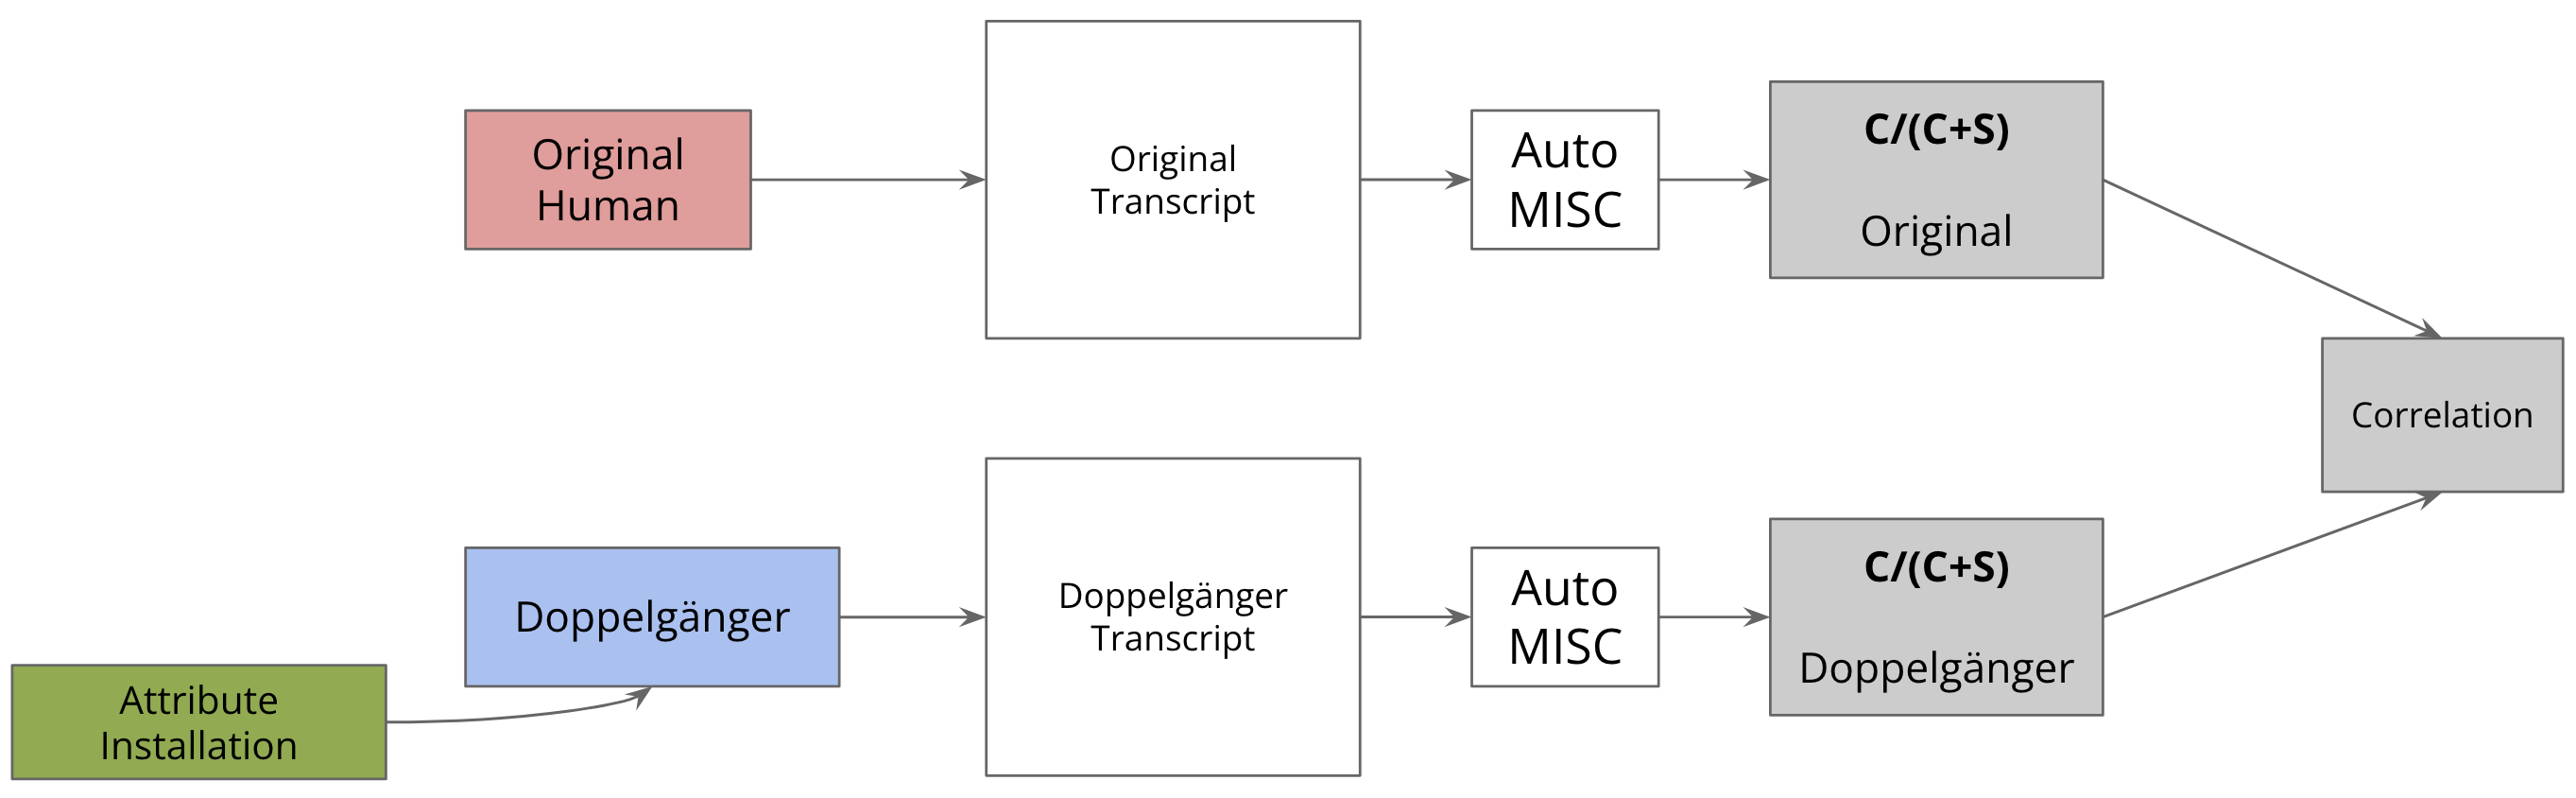
\includegraphics[width=0.98\textwidth]{fig/doppelganger_process.png}
    \caption{The doppelgänger creation and validation process. For each human participant ($H_i$), a synthetic twin ($S_i$) is created by installing their attributes ($A_{H_i}$). Both agents' conversations are analyzed to extract a behavioural metric (\%CT), and the correlation between the two sets of metrics is used to assess fidelity.}
    \label{fig:doppelgänger-creation-process}
\end{figure}


\subsubsection{Evaluation}
For each experiment with a set of attributes, we calculated the Spearman's correlation coefficient between the \%CT of human-MIBot doppelgänger-MIBot conversations.


% \subsubsection{Results}
% \begin{table}[ht!]
%     \centering
%     \begin{threeparttable}
%         \sisetup{
%             table-format=0.2,
%             table-space-text-post = $^{****}$
%         }
%         \renewcommand{\arraystretch}{1.2}
%         \caption{
%             Incremental attribute installation and its effect on the fidelity of doppelgängers. Fidelity is measured by the Spearman correlation of Percentage Change Talk (\%CT) between human participants and their doppelgängers (N=20). Each row represents a model where attributes were cumulatively added to the installation prompt.
%         }
%         \label{tab:doppelgänger-correlations}
%         \begin{tabular}{c cccccc S}
%             \toprule
%             \textbf{Experiment} & \multicolumn{6}{c}{\textbf{Installed Attributes}} & {\textbf{\makecell{Spearman's rank \\ correlation}}} \\
%             \cmidrule(r){2-7}
%             & \makecell{Pre-conv. \\ importance} & \makecell{Pre-conv. \\ readiness} & Age & Sex & \makecell{Pre-conv. \\ confidence} & \%CT & {$r_s$} \\
%             \midrule
%             1 & \checkmark & & & & & & 0.19 \\
%             2 & \checkmark & \checkmark & & & & & 0.24 \\
%             3 & \checkmark & \checkmark & \checkmark & & & & 0.26 \\
%             4 & \checkmark & \checkmark & \checkmark & & & & 0.40 \\
%             5 & \checkmark & \checkmark & \checkmark & \checkmark & & & 0.22\tnote{*} \\
%             6 & \checkmark & \checkmark & \checkmark & \checkmark & \checkmark & \checkmark & 0.57\tnote{****} \\
%             \bottomrule
%         \end{tabular}
%         \begin{tablenotes}
%             \footnotesize
%             \item[*] $p < 0.05$
%             \item[**] $p < 0.01$
%             \item[***] $p < 0.001$
%             \item[****] $p < 0.0001$
%         \end{tablenotes}
%     \end{threeparttable}
% \caption{Incremental attribute installation and its effect on the fidelity of doppelgängers. Fidelity is measured by the Spearman correlation of Percentage Change Talk (\%CT) between human participants and their doppelgängers (N=20). Each row represents a model where attributes were cumulatively added to the installation prompt.}
% \label{tab:doppelgänger-correlations}
% \end{table}

% \cref{tab:doppelgänger-correlations} shows the Spearman's rank correlation coefficient between \%CT of human-human and doppelgänger-human transcripts. Incremental installation of attributes does not always lead to an increase in the correlation coefficient. For example, adding pre-conversation confidence to the set of attributes made the correlation drop from 0.40 to 0.22. 

% We also installed \%CT as an attribute to test whether the doppelgängers could calibrate their change talk based on being numerically told their \%CT. As experiment $\# 6$ shows, after installing \%CT,  the doppelgänger modulated their behaviour and maintained a proportion of Change and Sustain talk coincident with the installed \%CT. This is perhaps the most surprising observation of this experiment.

% At the population level, analysis revealed discrepancies. The mean \%CT for doppelgängers (0.76) was substantially higher than that of the original human participants (0.59). This suggests that while the doppelgängers as a group could exhibit relative differences in motivational language, they were generally more inclined towards change talk than their human counterparts.

% Other observations we made during our experiments with incremental installation of attributes include:

% \begin{enumerate}
%     \item Once an attribute (e.g., pre-conversation importance) is installed in the doppelgängers, it is accurately recalled when prompted.

%     \item Asking the doppelgängers to think before filling up the post-conversation readiness rulers reduced the gap (as measured by MAE) between their and human-reported scores.

%     \item Uniform fidelity: Although the human-MIBot \%CT for both females and males were equal, the Spearman's correlation coefficient were markedly different (0.5 for females; 0.65 for males), necessitating further investigation into whether the synthetic smokers exhibited uniform fidelity for both sexes. 
% \end{enumerate}





% \begin{figure}[ht!]
%     \centering
%     \begin{minipage}{0.8\textwidth}
%         \centering
%         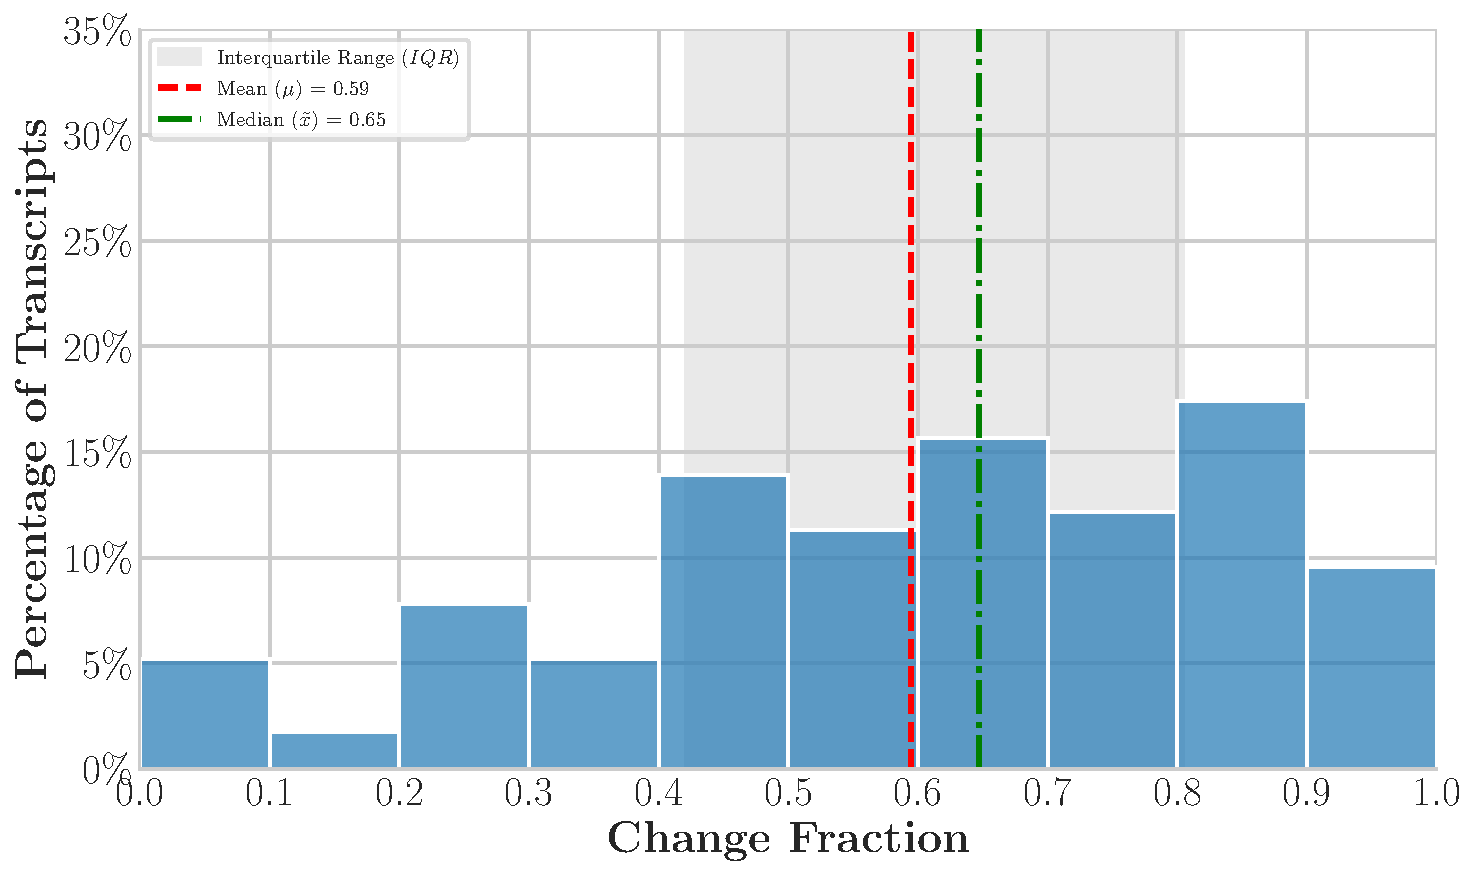
\includegraphics[width=\linewidth]{fig/change_frac_human_histogram.pdf}
%         \subcaption{Change Fraction for human-MIBot conversations}
%     \end{minipage}\vfill
%     \begin{minipage}{0.8\textwidth}
%         \centering
%         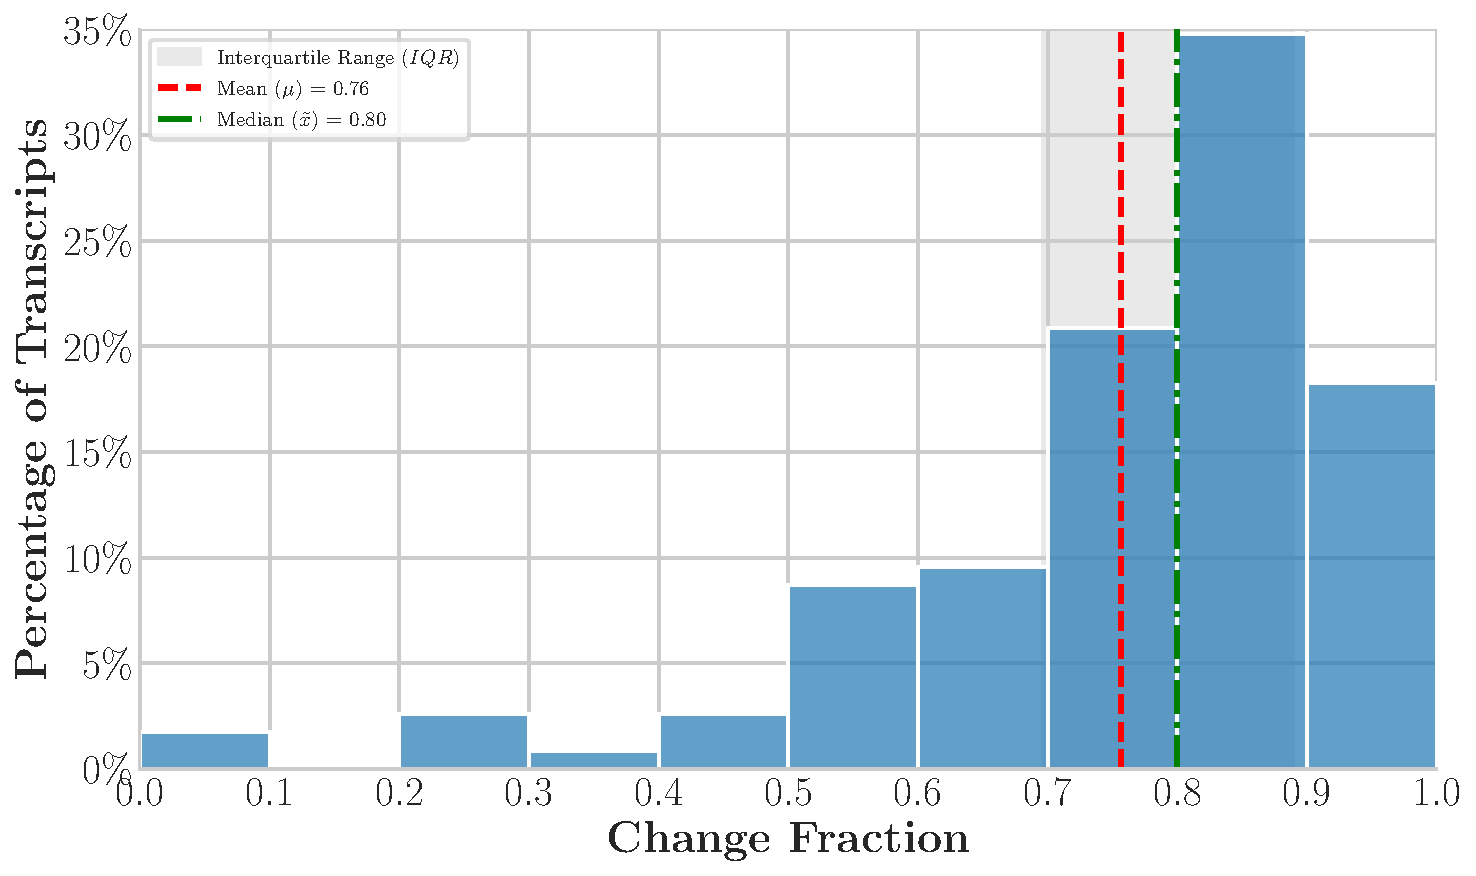
\includegraphics[width=\linewidth]{fig/change_frac_histogram.pdf}
%         \subcaption{Change Fraction for doppelgänger-MIBot conversations}
%     \end{minipage}
%     \caption{Distribution of Change Fraction (CF) for \textbf{(a)} human-MIBot and \textbf{(b)} doppelgänger-MIBot conversations. Change Fraction (CF) = \%CT$/100$. doppelgängers tend to exhibit high CF compared to their human twins.}
%     \label{fig:cf_comparison}
% \end{figure}


% \begin{figure}[ht!]
%     \centering
%     \includegraphics[width=0.7\textwidth]{fig/cf_doppelgänger_human.pdf}
%     \caption{Scatter plot of Change Fraction for human-MIBot \textbf{(x-axis)} and doppelgänger-MIBot \textbf{(y-axis)} conversations}
%     \label{fig:cf_human_vs_doppel}
% \end{figure}


% \begin{table}[ht!]
% \centering
% \begin{threeparttable}
% \label{tab:doppelgänger-fidelity-sex}
% \begin{tabular}{@{}lcccc@{}}
% \toprule
% \textbf{} & \textbf{} & \textbf{Human} & \textbf{Doppelgänger} & \textbf{Spearman's} \\

% \textbf{Group} & \textbf{N} & \textbf{\%CT} & \textbf{\%CT} & \textbf{Correlation} \\

% \textbf{} & \textbf{} & \textbf{Mean (SD)} & \textbf{Mean (SD)} & \textbf{($r_s$)} \\
% \midrule
% Male & 53 & 0.60 (0.27) & 0.77 (0.14) & 0.65\tnote{****} \\
% Female & 62 & 0.59 (0.25) & 0.75 (0.22) & 0.52\tnote{****} \\
% \bottomrule
% \end{tabular}
% \begin{tablenotes}
%     \item[****] \footnotesize $p < 0.0001$.
% \end{tablenotes}
% \end{threeparttable}
% \caption{Fidelity of doppelgänger's motivational language stratified by sex. Fidelity is measured by the Spearman correlation between the Percentage Change Talk (\%CT) of human participants and their corresponding doppelgängers.}
% \end{table}




% REPLACE the entire "Results" subsection with this new version.
\subsubsection{Results}
The results of the incremental attribute installation are summarized in Table~\ref{tab:doppelgänger-correlations}. The fidelity, measured as the Spearman's rank correlation between the \%CT of humans and their doppelgängers, evolved as more attributes were added. Initially, adding attributes like pre-conversation importance and readiness led to a gradual increase in correlation. However, the process was not strictly monotonic; for instance, adding `pre-conversation confidence' in experiment 5 unexpectedly lowered the correlation from 0.40 to 0.22.

The most significant finding emerged in experiment 6, where explicitly installing the human's \%CT value as a numerical instruction resulted in a strong and statistically significant correlation of $r_s = 0.57$ ($p < 0.0001$). This suggests an LLM-based doppelgänger can directly operationalize a behavioural target when provided, modulating its language to match a specified proportion of change versus sustain talk.

However, despite achieving a strong rank correlation, a closer look at the population-level statistics reveals a systematic bias. As shown in the histograms in Figure~\ref{fig:cf_comparison}, the distribution of \%CT for doppelgängers is shifted significantly higher than for humans (mean 0.76 vs. 0.59). The doppelgänger distribution is also more compressed and left-skewed, indicating a lower variance and a strong tendency to produce high levels of change talk, regardless of the human baseline.

This discrepancy is further visualized in the scatter plot in Figure~\ref{fig:cf_human_vs_doppel}. While the points follow a positive trend that confirms the correlation, the majority lie above the identity line ($y=x$). This visually demonstrates that doppelgängers consistently over-produced change talk relative to their human counterparts. Even when a human participant had a low \%CT (e.g., below 0.4), their doppelgänger often produced a \%CT above 0.6.

Finally, we investigated the system's uniform fidelity by stratifying the results by sex, as detailed in Table~\ref{tab:doppelgänger-fidelity-sex}. While the mean \%CT for both human males and females was nearly identical ($\approx$59\%), the fidelity of their doppelgängers differed. The correlation for males ($r_s = 0.65$) was notably stronger than for females ($r_s = 0.52$), indicating a performance bias. This lack of uniform fidelity suggests the model may simulate one demographic group more accurately than another, an issue requiring further investigation to ensure representative synthetic populations. Other observations include:

\begin{enumerate}
    \item Once an attribute (e.g., pre-conversation importance) is installed in the doppelgängers, it is accurately recalled when prompted.
    \item Asking the doppelgängers to think before filling up the post-conversation readiness rulers reduced the gap (as measured by MAE) between their and human-reported scores.
\end{enumerate}



\begin{table}[ht!]
    \centering
    \begin{threeparttable}
    \sisetup{
        table-format=0.2,
        table-space-text-post = $^{****}$
    }
    \renewcommand{\arraystretch}{1.2}
    \begin{tabular}{c cccccc S}
        \toprule
        \textbf{Experiment} & \multicolumn{6}{c}{\textbf{Installed Attributes}} & {\textbf{\makecell{Spearman's rank \\ correlation}}} \\
        \cmidrule(r){2-7}
        & \makecell{Pre-conv. \\ importance} & \makecell{Pre-conv. \\ readiness} & Age & Sex & \makecell{Pre-conv. \\ confidence} & \%CT & {$r_s$} \\
        \midrule
        1 & \checkmark & & & & & & 0.19 \\
        2 & \checkmark & \checkmark & & & & & 0.24 \\
        3 & \checkmark & \checkmark & \checkmark & & & & 0.26 \\
        4 & \checkmark & \checkmark & \checkmark & \checkmark & & & 0.40 \\
        5 & \checkmark & \checkmark & \checkmark & \checkmark & \checkmark & & 0.22\tnote{*} \\
        6 & \checkmark & \checkmark & \checkmark & \checkmark & \checkmark & \checkmark & 0.57\tnote{****} \\
        \bottomrule
    \end{tabular}
    \begin{tablenotes}
        \footnotesize
        \item[*] $p < 0.05$
        \item[**] $p < 0.01$
        \item[***] $p < 0.001$
        \item[****] $p < 0.0001$
    \end{tablenotes}
    \end{threeparttable}
        \caption{
        Incremental attribute installation and its effect on the fidelity of doppelgängers. Fidelity is measured by the Spearman correlation of Percentage Change Talk (\%CT) between human participants and their doppelgängers (N=20). Each row represents a model where attributes were cumulatively added to the installation prompt.
    }
    \label{tab:doppelgänger-correlations}
\end{table}


\begin{figure}[ht!]
    \centering
    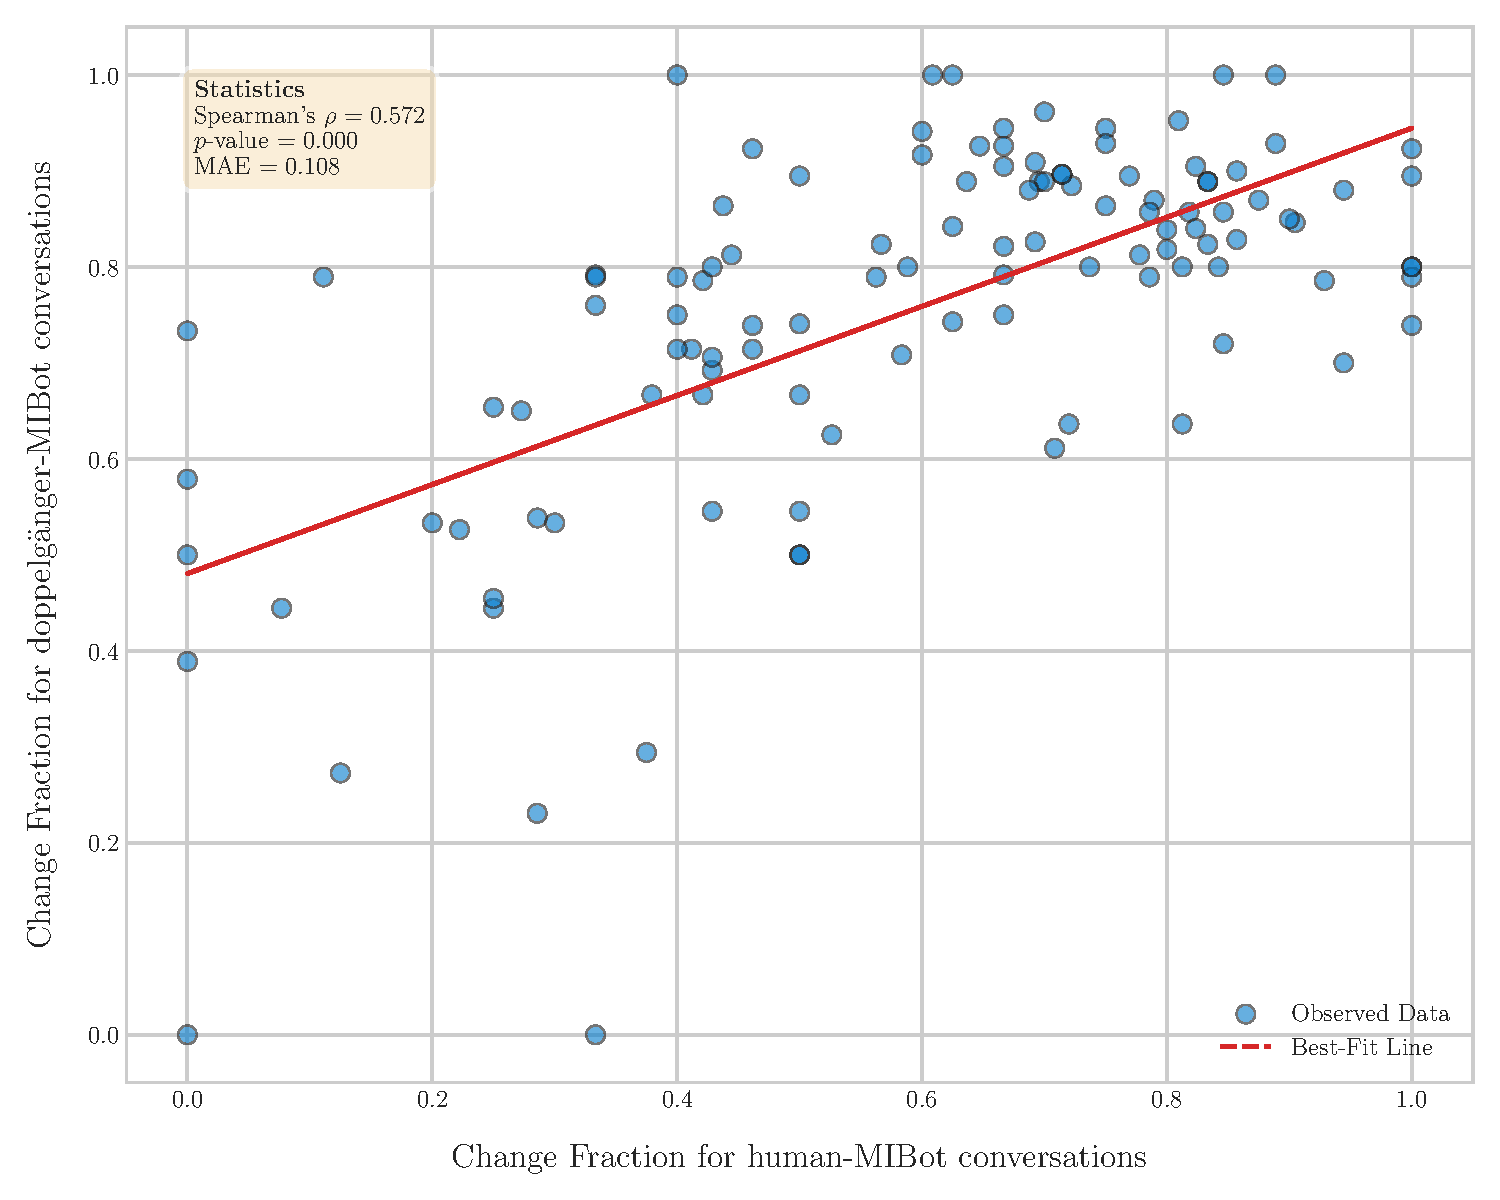
\includegraphics[width=0.7\textwidth]{fig/cf_doppelganger_human.pdf}
    \caption{Scatter plot of Change Fraction for human-MIBot \textbf{(x-axis)} and doppelgänger-MIBot \textbf{(y-axis)} conversations}
    \label{fig:cf_human_vs_doppel}
\end{figure}



\begin{figure}[ht!]
    \centering
    \begin{minipage}{0.8\textwidth}
        \centering
        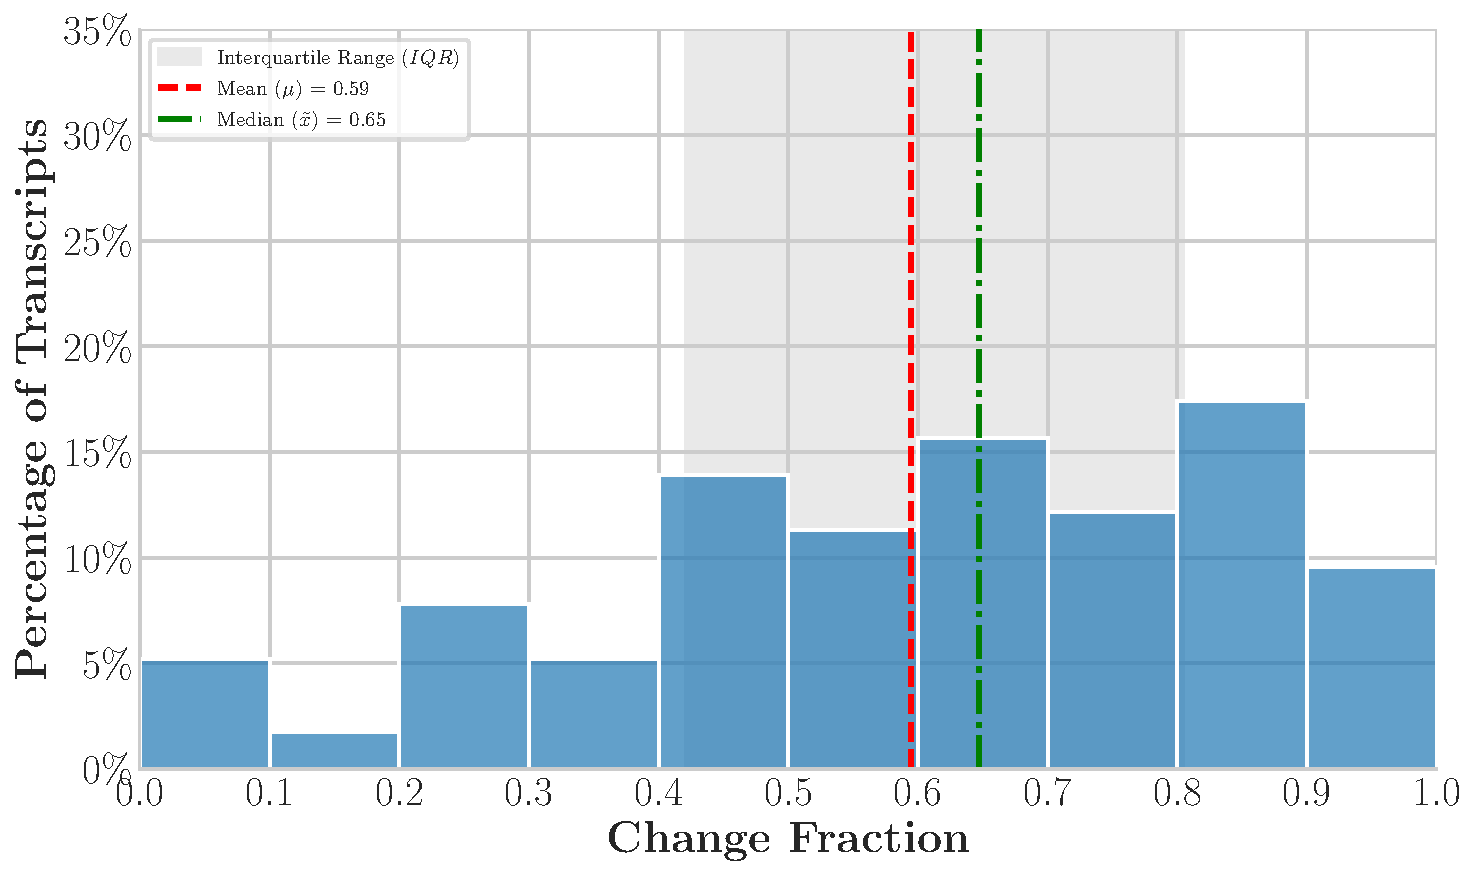
\includegraphics[width=\linewidth]{fig/change_frac_human_histogram.pdf}
        \subcaption{Change Fraction for human-MIBot conversations}
    \end{minipage}\vfill
    \begin{minipage}{0.8\textwidth}
        \centering
        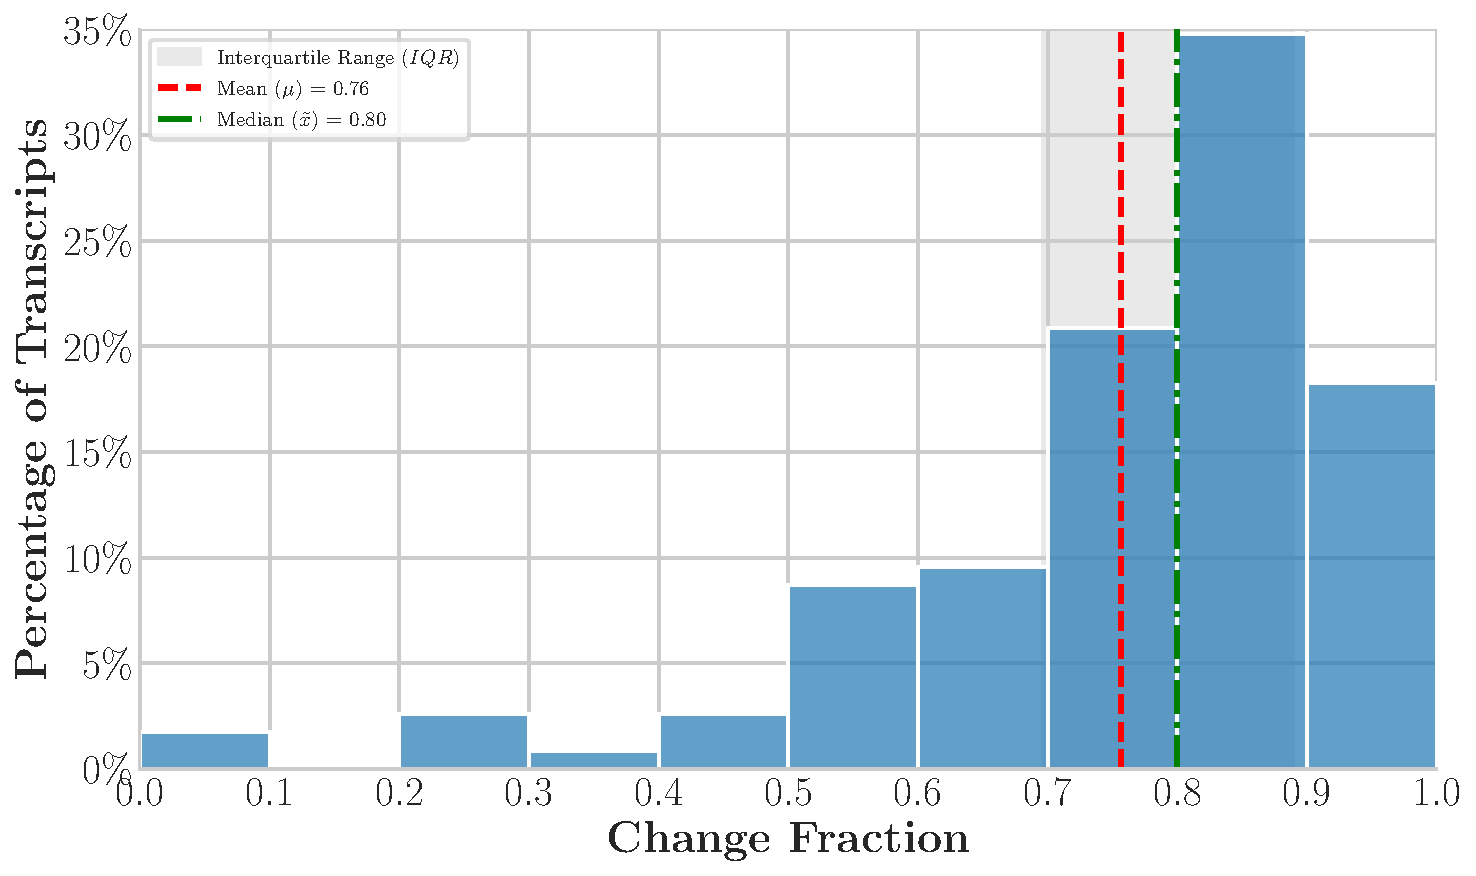
\includegraphics[width=\linewidth]{fig/change_frac_histogram.pdf}
        \subcaption{Change Fraction for doppelgänger-MIBot conversations}
    \end{minipage}
    \caption{Distribution of Change Fraction (CF) for \textbf{(a)} human-MIBot and \textbf{(b)} doppelgänger-MIBot conversations. Change Fraction (CF) = \%CT$/100$. doppelgängers tend to exhibit high CF compared to their human twins.}
    \label{fig:cf_comparison}
\end{figure}


\begin{table}[th!]
    \centering
    \begin{threeparttable}
        \begin{tabular}{@{}lcccc@{}}
        \toprule
        \textbf{} & \textbf{} & \textbf{Human} & \textbf{Doppelgänger} & \textbf{Spearman's} \\
        \textbf{Group} & \textbf{N} & \textbf{\%CT} & \textbf{\%CT} & \textbf{Correlation} \\
        \textbf{} & \textbf{} & \textbf{Mean (SD)} & \textbf{Mean (SD)} & \textbf{($r_s$)} \\
        \midrule
        Male & 53 & 0.60 (0.27) & 0.77 (0.14) & 0.65\tnote{****} \\
        Female & 62 & 0.59 (0.25) & 0.75 (0.22) & 0.52\tnote{****} \\
        \bottomrule
        \end{tabular}
        \begin{tablenotes}
            \item[****] \footnotesize $p < 0.0001$.
        \end{tablenotes}
    \end{threeparttable}
            \caption{Fidelity of doppelgänger's motivational language stratified by sex. Fidelity is measured by the Spearman correlation between the Percentage Change Talk (\%CT) of human participants and their corresponding doppelgängers.}
        \label{tab:doppelgänger-fidelity-sex}
\end{table}



\section{Evaluating the Utility of Synthetic Smokers}
\label{sec:synthetic-smoker-utility}

To assess the utility of synthetic smokers' in testing and training applications, an experiment was conducted to determine if they are sensitive to the quality of counselling they receive.

\subsection{Sensitivity to Counselling Quality}

Rationale: This experiment was designed to test whether synthetic smokers would exhibit differential responses when interacting with high-quality MI versus low-quality, confrontational counselling.

\subsubsection{Methodology}

\begin{enumerate}
    \item Sampling: Two participant groups (N=25 each) were created based on their actual Change Fraction (CF) in the MIBot study: a High-CF group (top 25th percentile) and a Low-CF group (bottom 25th percentile).

    \item Doppelgänger Creation: Doppelgängers were created for these 50 participants using the methodology described previously.
    
    \item Counsellor Conditions: These doppelgängers were exposed to two different automated counsellors:
    \begin{itemize}
        \item \textbf{Good MI Counsellor (MIBot v6.3A):} A high-quality, MI-adherent chatbot.
        
        \item \textbf{Bad (Confrontational) Counsellor:} An LLM prompted to be directive, judgmental, and confrontational (e.g., ``Giving advice without being asked,'' ``Trying to persuade them to quit...'').
    \end{itemize}
\end{enumerate}

\subsection{Evaluation}
We measured the Change Fraction (CF), the change in confidence after a simulated week ($\Delta$Confidence), and the CARE score as reported by the doppelgängers.

\subsubsection{Results}

\begin{table}[ht!]
\centering

\begin{tabular}{@{}llccc@{}}
\toprule
\textbf{Counsellor} & \textbf{Participant Group} & \textbf{CF} & \textbf{$\Delta$Confidence} & \textbf{CARE} \\ \midrule
\multirow{2}{*}{Good (MIBot 6.3A)} & High-CF Doppelgängers & 0.80 & 1.4 & 49.8 \\
& Low-CF Doppelgängers & 0.48 & 1.1 & 47.8 \\ \midrule
\multirow{2}{*}{Bad (Confrontational)} & High-CF Doppelgängers & 0.68 & 1.1 & 41.0 \\
& Low-CF Doppelgängers & 0.22 & 0.5 & 23.0 \\ \bottomrule
\end{tabular}
\caption{Doppelgänger outcomes when interacting with Good (MIBot 6.3A) vs. Bad (Confrontational) automated counsellors.}
\label{tab:good-vs-bad-counselling}
\end{table}

The results, shown in Table~\ref{tab:good-vs-bad-counselling}, indicate that the synthetic smokers were sensitive to counselling quality. When interacting with the Bad Counsellor, outcomes were significantly worse across all metrics. The Change Fraction (CF) dropped markedly, particularly for the Low-CF group (from 0.48 to 0.22), suggesting increased resistance. The Change in Confidence was lower, and the CARE scores showed a pronounced difference (e.g., 23.0 vs. 47.8 for the Low-CF group).

These findings suggest that the synthetic doppelgängers react in a predictable manner, responding negatively to poor-quality counselling. This sensitivity highlights their potential utility as evaluation and training tools.

\section{Conclusion}

This chapter detailed the development and validation of synthetic smokers, using a data-driven doppelgänger approach. The experiments showed that installing pre-conversation readiness rulers was a key factor in aligning the doppelgänger’s self-reported outcomes with those of their human counterparts. The conversational impact modelling and incremental attribute installation experiments resulted in high correlations between synthetic and human data. Notably, the explicit installation of a participant's Change Fraction value led to the doppelgänger's conversational output correlating strongly with the human data (Spearman’s $r_s = 0.57$).

However, the process also revealed several challenges. For example, the correlation of CARE scores was negligible, and a population-level bias was observed, with doppelgängers generally exhibiting higher average Change Talk than humans.

The validation experiments demonstrated that the doppelgängers are sensitive to the quality of motivational interviewing. They reacted differently to high-fidelity MI compared to confrontational counselling, showing reduced positive outcomes and lower perceived empathy scores when faced with poor therapeutic techniques. This sensitivity suggests the potential of synthetic smokers as a tool for the continued development and optimization of MIBot, and for providing feedback to novice MI counsellors on their skills.